\chapter{Results \& Evaluation}
\label{ch:Results and Evaluation}

This chapter describes the evaluation tests performed on the proposed approach on the basis of developed framework. Following sections are intended to give information about input data preparation, present and discuss obtained results. To start with, the trajectories approximation using polynomial regression is considered. After that the accuracy of clustering step is tested using an aforementioned DI index. As a conclusion, output results of a classification step are discussed, validation of the anomalies detection quality is done.

\section{Evaluation of Correctness and Accuracy}

This section gives details about evaluation tests performed to validate the accuracy of obtained results.

\subsection{Results of Trajectories Approximation using Polynomial Regression}

To make a decision about degrees of approximation polynomials, several experiments were run trying to fit the input trajectories into polynomials of 3\up{rd}, 4\up{th}, 5\up{th} degrees respectively. The following table depicts minimum and average values of $R^2$ metric for each of the experiments (Table \ref{table:r2_res}). 

\begin{table}[htb!]
	\caption{$R^2$ values for different degrees of polynomials}
	\label{table:r2_res}
	
	\setlength{\tabcolsep}{10pt}
	\centering
	\begin{tabular}[c]{|| C{2cm} | C{2cm} C{2cm} | C{2cm} C{2cm} ||} 
		\hline
		\multirow{3}{7em}{Degrees of polynomials} 	& \multicolumn{4}{c||}{$R^2$ score} \\[1ex]\cline{2-5}
		& \multicolumn{2}{c|}{X}	& \multicolumn{2}{c||}{Y} \\ [0.5ex]
		& min 	& avg				& min 	& avg \\ [0.5ex]
		\hline \hline
		\rowcolor{nogray} \multicolumn{5}{||c||}{$1.txt$ (before filtering)} \\ [0.5ex]
		\hline
		\{3\} 							& 0.66 	& 0.994 & 0.466 & 0.989 \\ [2ex]
		\rowcolor{backgray} \{3, 4\} 	& 0.897 & 0.998 & 0.823 & 0.994 \\ [2ex]
		\{3, 4, 5\} 					& 0.949 & 0.998 & 0.864 & 0.995 \\ [2ex]
		
		\hline \hline
		\rowcolor{nogray} \multicolumn{5}{||c||}{$1.txt$} \\ [0.5ex]
		\hline
		\{3\} 							& 0.689 & 0.997 & 0.777 & 0.995 \\ [2ex]
		\rowcolor{backgray} \{3, 4\} 	& 0.942 & 0.999 & 0.872 & 0.997 \\ [2ex]
		\{3, 4, 5\} 					& 0.98 	& 0.999 & 0.88 	& 0.997 \\ [2ex]
		
		\hline \hline
		\rowcolor{nogray} \multicolumn{5}{||c||}{$2.txt$} \\ [0.5ex]
		\hline
		\{3, 4\} 						& 0.992 & 0.9997 & 0.832 & 0.996 \\ [2ex]
		\hline \hline
		
		\rowcolor{nogray} \multicolumn{5}{||c||}{$3.txt$} \\ [0.5ex]
		\hline
		\{3, 4\} 						& 0.815 & 0.995 & 0.867 & 0.996 \\ [2ex]
		\hline \hline
		
		\rowcolor{nogray} \multicolumn{5}{||c||}{$4.txt$} \\ [0.5ex]
		\hline
		\{3, 4\} 						& 0.879 & 0.995 & 0.722 & 0.993 \\ [2ex]
		\hline
	\end{tabular}
\end{table}

This paragraph will discuss results of experiments using trajectories from first intersection ($1.txt$) before and after filtering the trajectories. It can be seen from the Table \ref{table:r2_res} that the average values of $R^2$ score are acceptable for all the experiments. However, the minimum $R^2$ values, which are equal to 0,66 and 0,466 for the first experiment with only 3\up{rd}-degree polynomials for unfiltered trajectories, are poor and unsatisfactory, meaning that model can predict barely half of the points for some trajectories correctly. Filtering out trajectories with short displacements in terms of both space and time improved the results significantly. However, results for approximation using 3\up{rd}-degree polynomials are still insufficient. This can affect following analysis and worsen further analysis. For that reason approximation using several degrees was performed in a following way:

\begin{enumerate}
	\setlength\itemsep{0em}
	\item firstly perform approximation using the lowest degree of a polynomial as a starting point,
	\item compare the obtained $R^2$ with a predefined threshold (0,98 in this case); if the obtained value is less than the threshold value, increase the degree and reperform polynomial regression,
	\item continue till the acceptable $R^2$ is obtained or till reaching the limit for a polynomial degree to check (5 in this case). 
\end{enumerate} 

Approximation using 3\up{rd} and 4\up{th} degree polynomials in conjunction improved both minimum and average values of $R^2$ drastically. Though adding a 5\up{th} degree polynomial into consideration did not affect results significantly and improved the average coefficient only for 0,01 in comparison with the previous experiment. In view of this it was decided to focus on approximation using 3\up{rd} and 4\up{th} degrees and run the experiments on rest of input trajectories data sets ($2.txt$, $3.txt$, $4.txt$).

For the sake of simplicity the trajectories are classified into two groups depending on a degree of polynomials used to approximate: first group contains trajectories approximated with a 3\up{rd} degree polynomial functions while the second group consists of trajectories approximated with a 4\up{th} degree polynomial functions. Both groups were analyzed in terms of a shape and an average speed. Figure \ref{fig:regr-pol-4} depicts second group of trajectories and Table \ref{table:speeds} gives the minimum, average and maximum speed of trajectories for both groups.

\begin{figure}[!htb]
	\centering
	\begin{subfigure}[!htb]{0.3\textwidth}
		\centering{}
		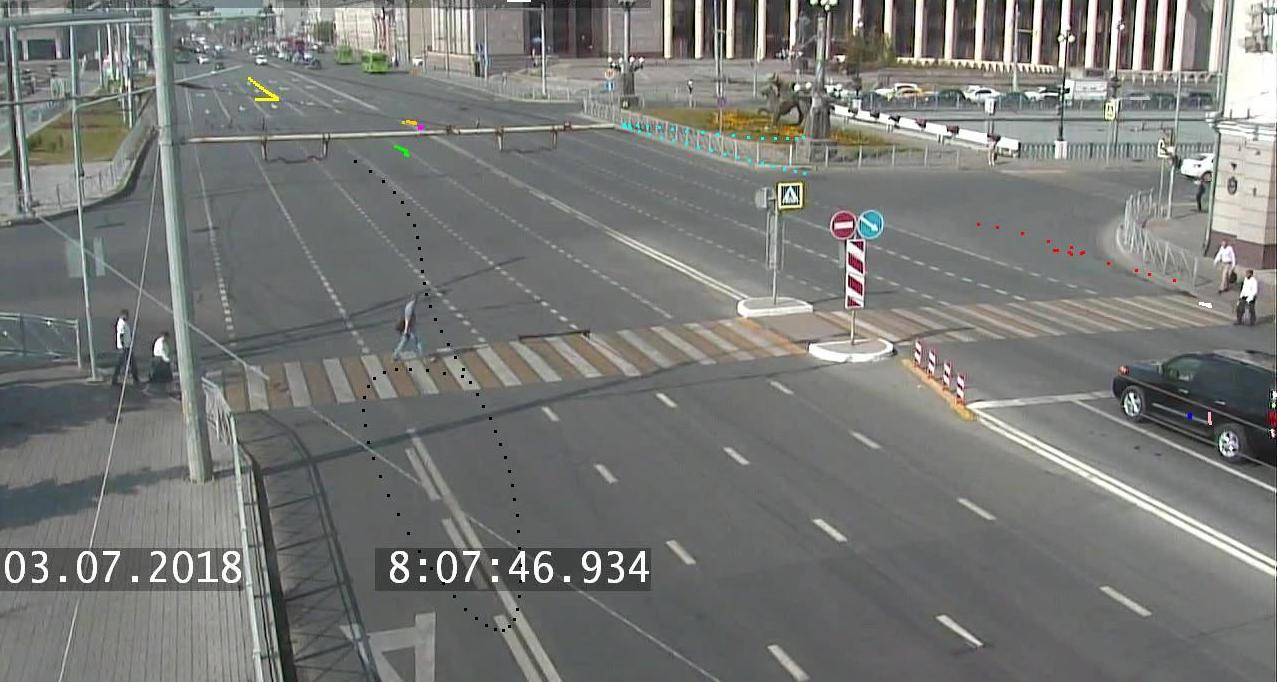
\includegraphics[width=\textwidth]{images/regr_1_pol_4.jpg}
		\caption{$1.txt$}
		\label{fig:regr-1-pol-4}
	\end{subfigure}
	\hfill
	\begin{subfigure}[!htb]{0.3\textwidth}
		\centering{}
		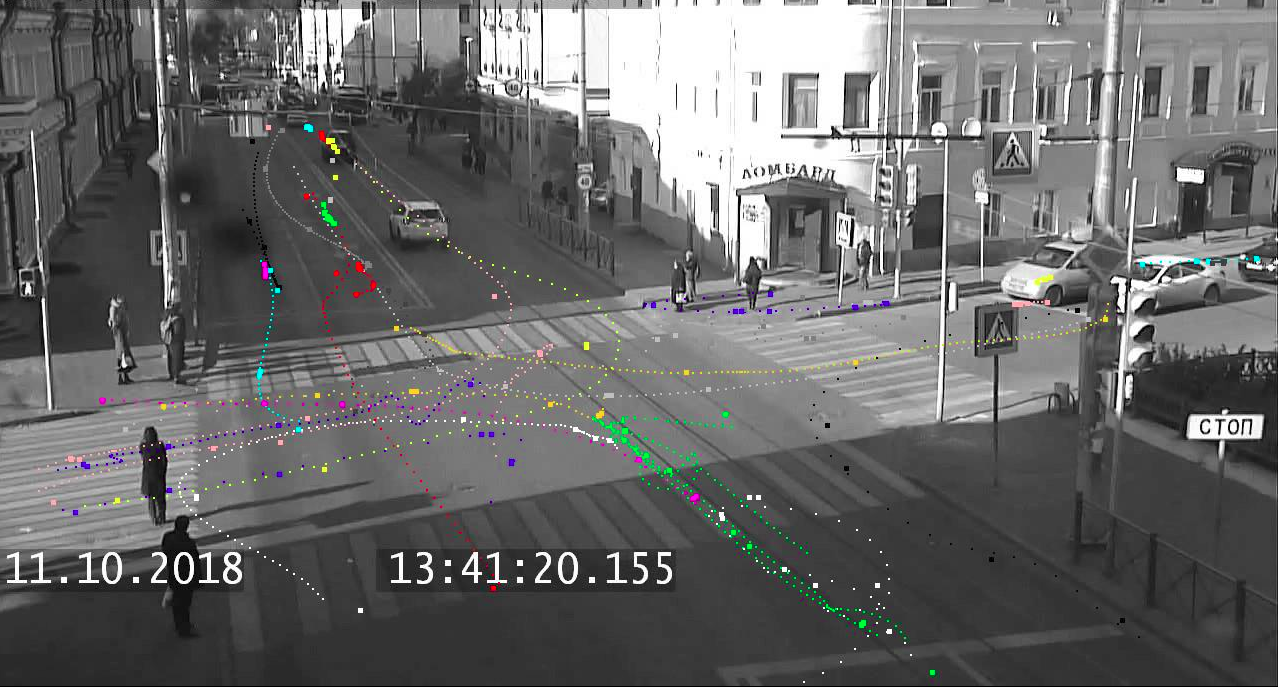
\includegraphics[width=\textwidth]{images/regr_3_pol_4.png}
		\caption{$3.txt$}
		\label{fig:regr-3-pol-4}
	\end{subfigure}
	\hfill
	\begin{subfigure}[!htb]{0.3\textwidth}
		\centering{}
		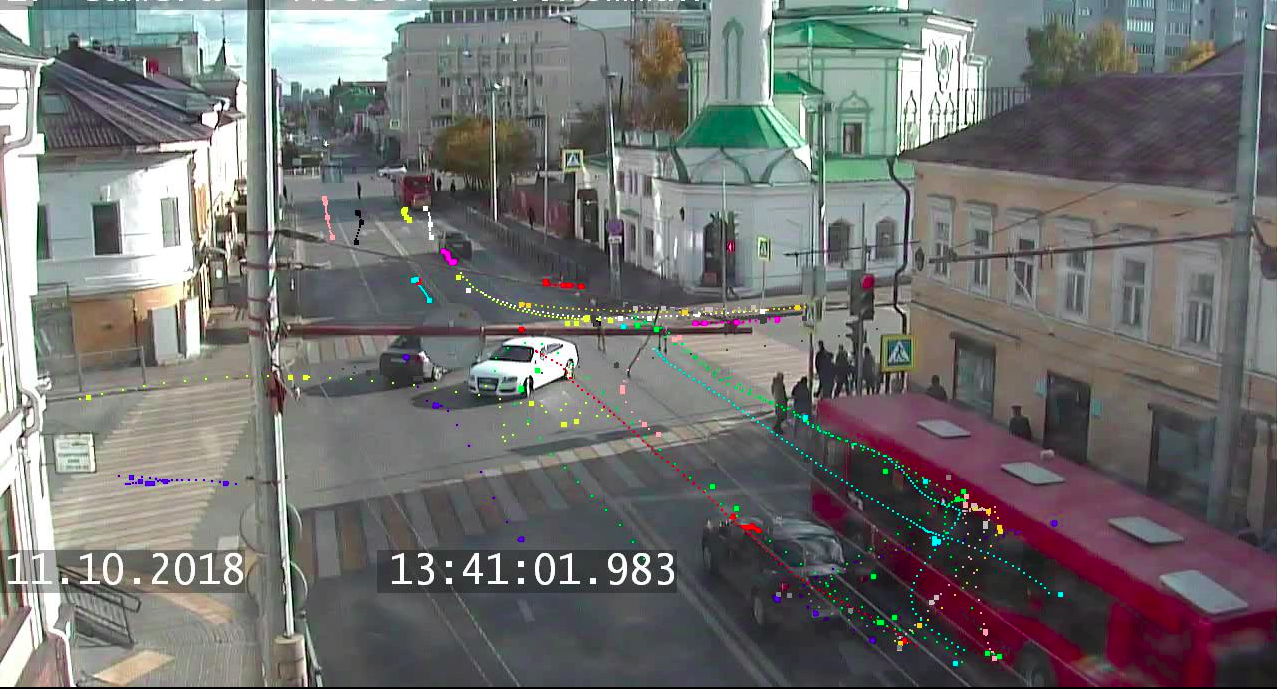
\includegraphics[width=\textwidth]{images/regr_4_pol_4.png}
		\caption{$4.txt$}
		\label{fig:regr-4-pol-4}
	\end{subfigure}
	\caption{Trajectories approximated with 4\up{th}-degree polynomial functions}
	\label{fig:regr-pol-4}
\end{figure}

\begin{table}[htb!]
	\caption{Overview of min, avg and max speeds of vehicles}
	\label{table:speeds}
	
	\setlength{\tabcolsep}{10pt}
	\centering
	\begin{tabular}[c]{|| C{2.5cm} | C{2.5cm} C{2.5cm} C{2.5cm} ||} 
		\hline
		\multirow{2}{7em}{Degree of a polynomial} 	
		& \multicolumn{3}{c||}{Speed \textit{(pixels per sec)}} \\[1ex]\cline{2-4}
		& min 		& avg		& max 				\\ [2ex]
		
		\hline \hline
		\rowcolor{nogray} \multicolumn{4}{||c||}{$1.txt$ (before filtering)} 	\\ [0.5ex]
		\hline
		\rowcolor{backgray} \{3\} 	& 18.555 	& 335.365 	& 1721.499 			\\ [2ex]
		
		\rowcolor{backgray} \{4\} 	& 1.206		& 72.34 	& 374.396 			\\ [2ex]
		\hline
		
		\rowcolor{nogray} \multicolumn{4}{||c||}{$1.txt$} 	\\ [0.5ex]
		\hline
		\rowcolor{backgray} \{3\} 	& 61.814 	& 372.435 	& 909.121 			\\ [2ex]
		
		\rowcolor{backgray} \{4\} 	& 26.603	& 229.053 	& 602.773 			\\ [2ex]
		
		\hline
		\rowcolor{nogray} \multicolumn{4}{||c||}{$2.txt$} 	\\ [0.5ex]
		\hline
		\{3\} 	& 85.705 	& 494.016 	& 1107.96 			\\ [2ex]
		
		\{4\} 	& 183.087	& 613.865 	& 900.737 			\\ [2ex]
		\hline
		
		\rowcolor{nogray} \multicolumn{4}{||c||}{$3.txt$} 	\\ [0.5ex]
		\hline
		\{3\} 	& 13.65 	& 301.481 	& 1012.748 			\\ [2ex]
		
		\{4\} 	& 29.26		& 206.119 	& 764.25 			\\ [2ex]
		\hline
		
		\rowcolor{nogray} \multicolumn{4}{||c||}{$4.txt$} 	\\ [0.5ex]
		\hline
		\{3\} 	& 43.01 	& 269.074 	& 872.33	 		\\ [2ex]
		
		\{4\} 	& 22.92		& 163.431 	& 708.154 			\\ [2ex]
		\hline
		
	\end{tabular}
\end{table}

Thereinafter the trajectories approximated with 3\up{rd}- and 4\up{th}-degree polynomial functions will be referred to as a first and second groups of trajectories respectively. It can be observed that trajectories different groups have the widely differing speeds. The first group includes trajectories with much higher speeds, particularly striking is that the maximum speed for the second group is almost equal to average speed for the first group and the average speed for the first group is almost four times as much as for the second group for the case of unfiltered trajectories. After excluding the short trajectories from the consideration results became more smooth, however the same observation still takes place and is still noticeable. Also the picture depicts that 4\up{th}-degree polynomial functions were used to approximate trajectories of complex shape or trajectories with densely located trajectory points. 

Such a tendency is mostly distinguishable while considering trajectories from the first intersection, which can supposed to be the representative set of trajectories since it has the largest amount of data instances. It is also worth noting that the second trajectories data set ($2.txt$) has only 10 trajectories in the first group, hence the trajectories speed analysis can not be very accurate.

The results of performed polynomial regression approximation and key points calculation are presented in Figure \ref{fig:regr-kp111}. The original trajectory data is visualized using a red color, while the blue trajectory points correspond to data points obtained using the functions of a polynomial approximation for the same time points. Key points of each trajectory are emphasized using bold blue square dots. It can be seen that the approximation function is close to the original trajectory function, for some trajectories approximation gives the same coordinates as in the original data (for trajectories with approximation polynomials having $R^2 \approx 1.0$). Also key points accurately follow the approximation line and describe the trajectory properly, hence, they can be used instead of original trajectory points to simplify the further trajectories analysis. 

\begin{figure}[!htb]
	\centering
	\begin{subfigure}[!htb]{0.68\textwidth}
		\centering{}
		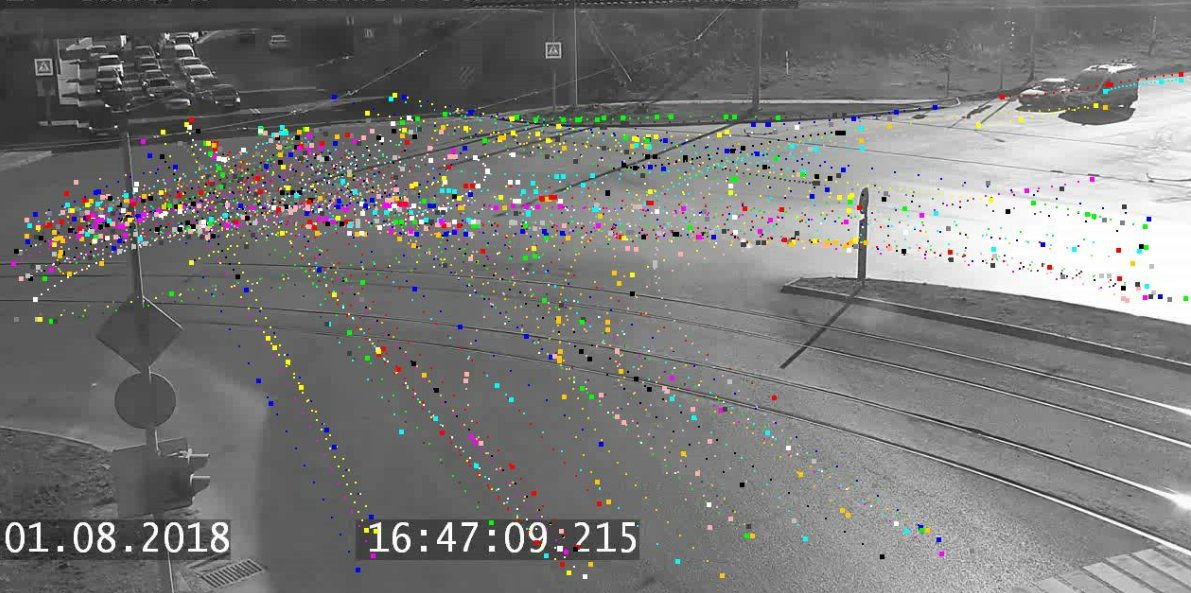
\includegraphics[width=\textwidth]{images/regr_kp_full.png}
		\caption{full $2.txt$}
	\end{subfigure}
	\hfill
	\begin{subfigure}[!htb]{0.3\textwidth}
		\centering{}
		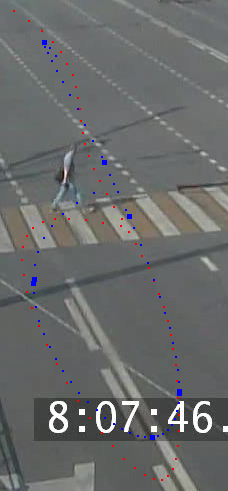
\includegraphics[width=\textwidth]{images/regr_kp_loop.png}
		\caption{loop from $1.txt$}
	\end{subfigure}
	\hfill
	\begin{subfigure}[!htb]{0.3\textwidth}
		\centering{}
		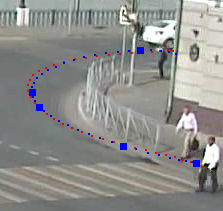
\includegraphics[width=\textwidth]{images/regr_kp_turn.png}
		\caption{turn from $1.txt$}
	\end{subfigure}
	\hfill
	\begin{subfigure}[!htb]{0.3\textwidth}
		\centering{}
		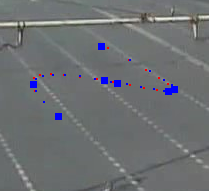
\includegraphics[width=\textwidth]{images/regr_kp_complex.png}
		\caption{complex $1.txt$}
	\end{subfigure}
	\hfill
	\begin{subfigure}[!htb]{0.3\textwidth}
		\centering{}
		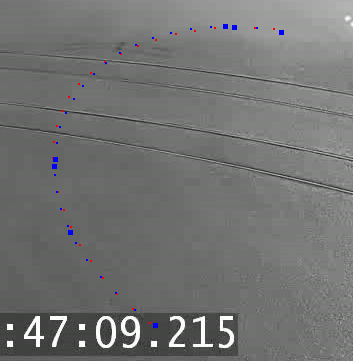
\includegraphics[width=\textwidth]{images/regr_kp_curve_2.png}
		\caption{curve from $2.txt$}
	\end{subfigure}
	\hfill
	\begin{subfigure}[!htb]{0.3\textwidth}
		\centering{}
		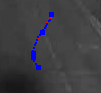
\includegraphics[width=\textwidth]{images/regr_kp_complex_3.png}
		\caption{complex from $3.txt$}
	\end{subfigure}
	\hfill
	\begin{subfigure}[!htb]{0.3\textwidth}
		\centering{}
		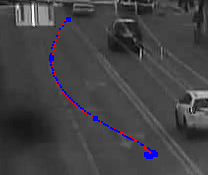
\includegraphics[width=\textwidth]{images/regr_kp_curve_3.png}
		\caption{curve from $3.txt$}
	\end{subfigure}
	\hfill
	\begin{subfigure}[!htb]{0.3\textwidth}
		\centering{}
		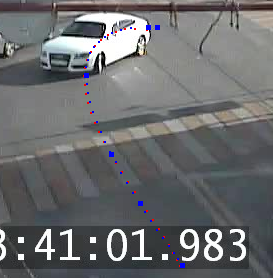
\includegraphics[width=\textwidth]{images/regr_kp_curve_4.png}
		\caption{curve from $4.txt$}
	\end{subfigure}
	
	\caption{Results of polynomial regression with emphasizing key points}
	\label{fig:regr-kp111}
\end{figure}

\subsubsection{Summary}

Hence, it follows up that the higher-order polynomial functions are preferred to approximate trajectories of following groups:

\begin{itemize}
	\setlength\itemsep{0em}
	\item slow-moving or inactive vehicle trajectories (including trajectories of vehicles waiting at the intersections), detectable on Figure \ref{fig:regr-1-pol-4};
	\item vehicle trajectories with a non-constant speed or an acceleration on some sections of a path (can be represented by non-equal allocation of trajectory points, where dense areas of trajectory points signalize about acceleration during these time intervals; as a result low-order polynomial can not describe such a complex dependency between a coordinate and a time);
	\item trajectories of complex shapes (sharp turns, Pascal snails), especially recognizable on Figures \ref{fig:regr-pol-4}b-c.
\end{itemize}

\subsection{Results of Trajectories Approximation using RDP Algorithm}

\subsubsection{Traditional RDP Algorithm}

Comparison of total length of approximated trajectories and the positional errors are presented in Table \ref{table:rdp_length_pos_err}. As it can be seen, starting from the $\varepsilon = 2.0$ approximation results are not usable. For the case of $\varepsilon = 2.0$ the average length of approximated trajectory is equal to the desired length, however many trajectories remain too long.

\begin{table}[htb!]
	\caption{Overview of min, avg and max length and positional errors for trajectories, approximated with RDP algorithm}
	\label{table:rdp_length_pos_err}
	
	\setlength{\tabcolsep}{9pt}
	\centering
	\begin{tabular}[c]{|| C{2cm} C{2cm} C{2cm} | C{2cm} C{2cm} C{2cm} ||} 
		\hline

		\multicolumn{3}{||c|}{Length \textit{(TPs)}} & \multicolumn{3}{c||}{Positional Error \textit{(pixels)}} \\[1ex]\cline{1-6}
		min 	& avg	& max	& min 	& avg	& max 	\\ [2ex]
		
		\hline \hline
		\multicolumn{6}{||c||}{$\varepsilon = 0.5$} 	\\ [0.5ex]
		2 		& 11 	& 43 	& 0.0 	& 3.1 	& 11.03 \\ [2ex]

		\hline
		\multicolumn{6}{||c||}{$\varepsilon = 1.0$} 	\\ [0.5ex]
		2 		& 6.4 	& 33 	& 0.0 	& 7.2 	& 30.68 \\ [2ex]

		\hline
		\multicolumn{6}{||c||}{$\varepsilon = 1.5$} 	\\ [0.5ex]
		2 		& 5.35 	& 31 	& 0.0 	& 10.26 & 39.24 \\ [2ex]

		\hline
		\multicolumn{6}{||c||}{$\varepsilon = 2.0$} 	\\ [0.5ex]
		2 		& 4.7 	& 24 	& 0.0 	& 14.1 	& 61.3 	\\ [2ex]

		\hline
		\multicolumn{6}{||c||}{$\varepsilon = 10.0$} 	\\ [0.5ex]
		2 		& 2.64 	& 13 	& 0.0 	& 72.117 	& 354.62 	\\ [2ex]

		\hline
		\multicolumn{6}{||c||}{$\varepsilon = 10.5$} 	\\ [0.5ex]
		2 		& 2.6 	& 12 	& 0.0 	& 77.66 	& 505.73 	\\ [2ex]

		\hline
		\multicolumn{6}{||c||}{$\varepsilon = 11.0$} 	\\ [0.5ex]
		2 		& 2.24 	& 7 	& 0.0 	& 137.31 	& 1035.12 	\\ [2ex]
		
		\hline
		
	\end{tabular}
\end{table}

However, notwithstanding that traditional RDP algorithm chooses adequate, representative points, it does not guarantee the exact amount of resulting points. Moreover, for trajectories of vehicles moving in a straightforward direction, meaning all original \textit{TPs} are on a straight line, RDP algorithm will keep only first and last points. Such a behavior describes the trajectory form accurately, but do not appropriate to use for clustering. That leads to the necessity to perform a completion of approximation points by calculating additional key points.

\subsubsection{Douglas-Peucker N Algorithm}

The same comparison is performed for the Douglas-Peucker N Algorithm for different values of $N$, results are given in Table \ref{table:rdp_n_length_pos_err}. The minimum length is equal to 2, meaning that \textit{TPs} are located on a straight line, and the trajectory coincides with the initial simplifying line, consisting of the first and last trajectory points (Figure \ref{fig:rdp_2_points_only}). Notwithstanding that, the average length is almost equal to the desired $N$ value. Moreover, as expected, increase of $N$ value leads to the decrease of the positional error. 

Simplified trajectories obtained by applying the Douglas-Peucker N algorithm are presented in Figure \ref{fig:rdp-n-res} for the parameter value $N = 9$, representing the desired amount of simplification points.

\begin{figure}[!htb]
	\begin{subfigure}[!htb]{0.32\textwidth}
		\centering{}
		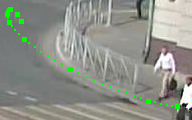
\includegraphics[width=\textwidth]{images/rdp-n-curve-1.png}
		\caption{curve from $1.txt$}
	\end{subfigure}
	\hfill
	\begin{subfigure}[!htb]{0.32\textwidth}
		\centering{}
		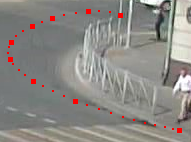
\includegraphics[width=\textwidth]{images/rdp-n-turn.png}
		\caption{turn from $1.txt$}
	\end{subfigure}
	\hfill
	\begin{subfigure}[!htb]{0.25\textwidth}
		\centering{}
		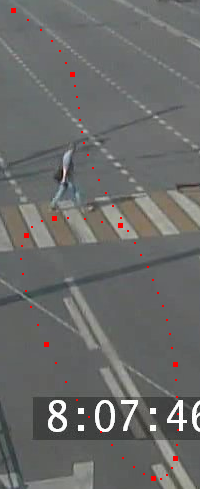
\includegraphics[width=\textwidth]{images/rdp-n-curve.png}
		\caption{loop from $1.txt$}
	\end{subfigure}
	\hfill
	\begin{subfigure}[!htb]{0.48\textwidth}
		\centering{}
		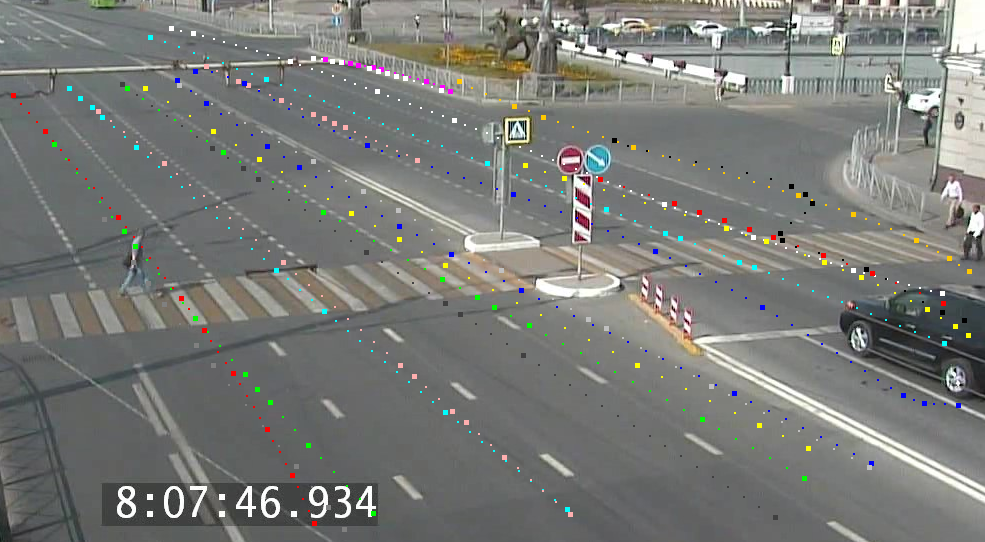
\includegraphics[width=\textwidth]{images/rdp-n-straight-before.png}
		\caption{straight trajectories $1.txt$}
	\end{subfigure}
	\hfill
	\begin{subfigure}[!htb]{0.48\textwidth}
		\centering{}
		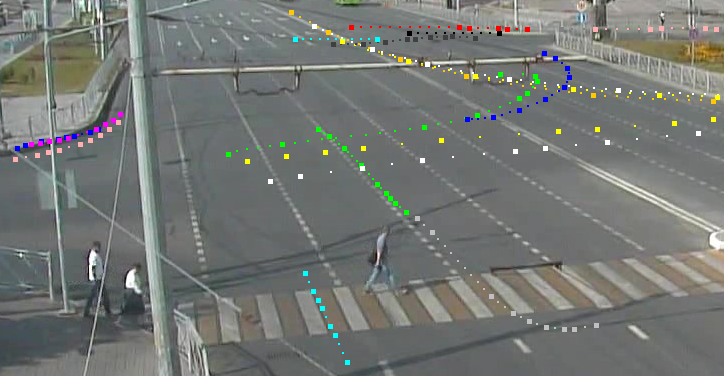
\includegraphics[width=\textwidth]{images/rdp-n-turns.png}
		\caption{turns from $1.txt$}
	\end{subfigure}
	\hfill
	\begin{subfigure}[!htb]{0.48\textwidth}
		\centering{}
		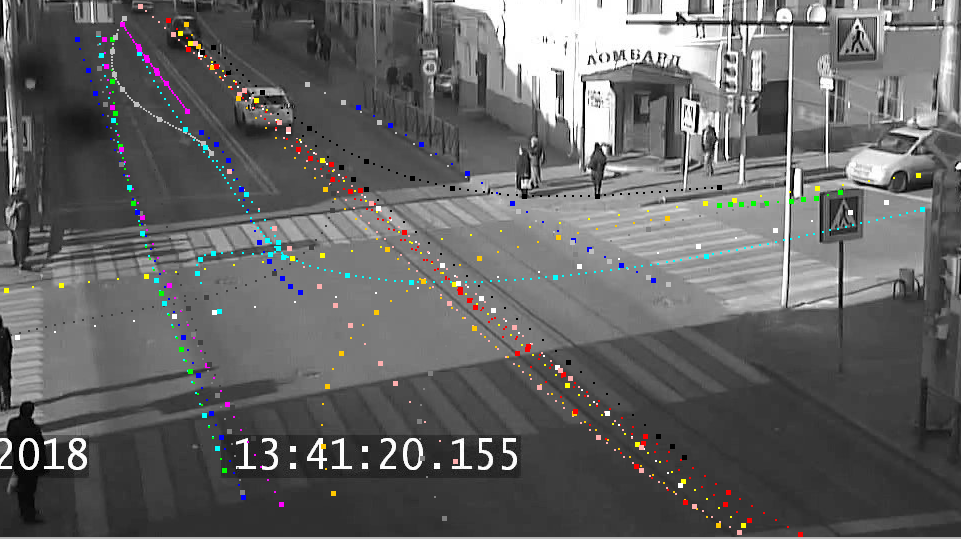
\includegraphics[width=\textwidth]{images/rdp-n-long-3.png}
		\caption{selection from $3.txt$}
	\end{subfigure}
	\hfill
	\begin{subfigure}[!htb]{0.48\textwidth}
		\centering{}
		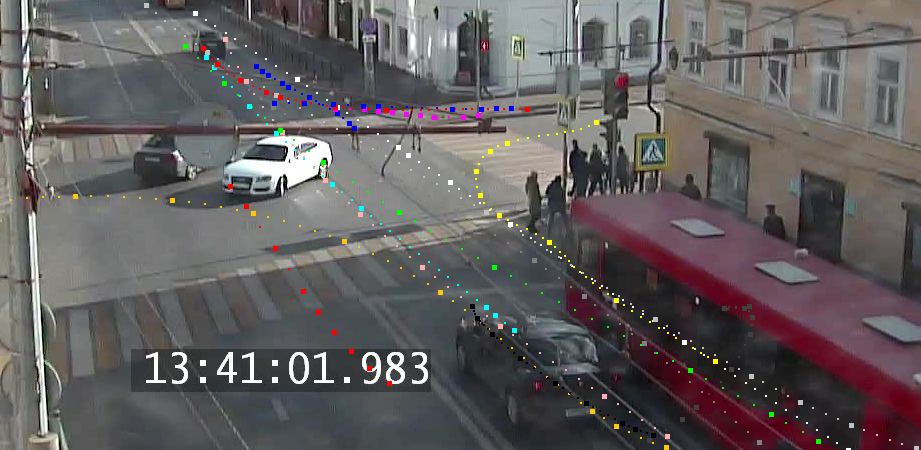
\includegraphics[width=\textwidth]{images/rdp-n-long-4.png}
		\caption{selection from $4.txt$}
	\end{subfigure}
	
	\caption{Results of Douglas-Peucker N simplification}
	\label{fig:rdp-n-res}
\end{figure}

Trajectories approximated by only first and last points will be complemented by calculating middle points to fulfill the desired maximum amount of \textit{TPs} in a simplified trajectory (Figure \ref{fig:rdp_2_points_filled}). Some of the points are redundant, but improve the clustering results.

\begin{figure}[!htb]
	\centering
	\begin{subfigure}[!htb]{0.9\textwidth}
		\centering{}
		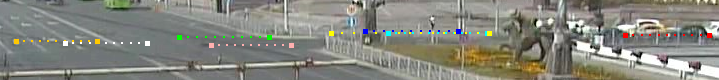
\includegraphics[width=\textwidth]{images/rdp-2-points.png}
		\caption{before adding middle points}
		\label{fig:rdp_2_points_only}
	\end{subfigure}
	\hfill
	\begin{subfigure}[!htb]{0.9\textwidth}
		\centering{}
		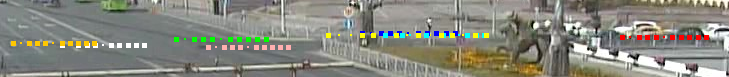
\includegraphics[width=\textwidth]{images/rdp-2-points-filled.png}
		\caption{complemented by middle points}
		\label{fig:rdp_2_points_filled}
	\end{subfigure}
	\caption{Douglas-Peucker N $3.txt$}
	\label{fig:rdp_2_points}
\end{figure}

\begin{table}[htb!]
	\caption{Overview of min, avg and max length and positional errors for trajectories, approximated with Douglas-Peucker N algorithm}
	\label{table:rdp_n_length_pos_err}
	
	\setlength{\tabcolsep}{10pt}
	\centering
	\begin{tabular}[c]{|| C{2cm} C{2cm} C{2cm} | C{2cm} C{2cm} C{2cm} ||} 
		\hline
		
		\multicolumn{3}{||c|}{Length \textit{(TPs)}} & \multicolumn{3}{c||}{Positional Error \textit{(pixels)}} \\[1ex]\cline{1-6}
		min 	& avg	& max	& min 	& avg	& max 	\\ [2ex]
		
		\hline \hline
		\multicolumn{6}{||c||}{$N = 7$} 	\\ [0.5ex]
		2 		& 6.86 	& 7 	& 0.0 	& 12.2 	& 472.36 \\ [2ex]

		\hline
		\multicolumn{6}{||c||}{$N = 8$} 	\\ [0.5ex]
		2 		& 7.82 	& 8 	& 0.0 	& 9.26 	& 388.85 \\ [2ex]

		\hline
		\multicolumn{6}{||c||}{$N = 9$} 	\\ [0.5ex]
		2 		& 8.76 	& 9 	& 0.0 	& 7.38 	& 340.56 \\ [2ex]
		
		\hline
		
	\end{tabular}
\end{table}

\subsubsection{Summary}

In order to choose between aforementioned implemented approximation methods, the obtained results need to be compared using the same accuracy evaluation method. For that the Positional errors metric was chosen. It can work with both algorithms, because Polynomial Regression, as well as Douglas-Peucker N, simplifies the input trajectory into a reduced number of key points. Positional error value demonstrates how far is the obtained simplified curve from the original.

Results of comparison are given in Table \ref{table:pr_dpn_comparison}. For trajectories approximated using a Polynomial Regression positional errors are calculated on the set of final key points, consisting of the solutions of derivative equations, border and middle points.

\begin{table}[htb!]
	\caption{Comparison of min, avg, max lengths and positional errors for trajectories, simplified by Polynomial Regression and Douglas-Peucker N algorithms}
	\label{table:pr_dpn_comparison}
	
	\setlength{\tabcolsep}{10pt}
	\centering
	\begin{tabular}[c]{|| C{2cm} C{2cm} C{2cm} | C{2cm} C{2cm} C{2cm} ||} 
		\hline
		
		\multicolumn{3}{||c|}{Length \textit{(TPs)}} & \multicolumn{3}{c||}{Positional Error \textit{(pixels)}} \\[1ex]\cline{1-6}
		min 	& avg	& max	& min 	& avg	& max 	\\ [2ex]
		
		\hline \hline
		\multicolumn{6}{||c||}{$1.txt$} 						\\ [0.5ex]
		\hline
		\multicolumn{6}{||c||}{Polynomial Regression, $N = 9$} 	\\ [0.5ex]
		6 		& 8.34 	& 9 	& 0.0 	& 29.18 	& 959.48 \\ [2ex]
		\hline
		\multicolumn{6}{||c||}{Douglas-Peucker N, $N = 9$} 	\\ [0.5ex]
		7 		& 8.97 	& 9 	& 0.0 	& 7.26 		& 340.56 \\ [2ex]
		
		\hline \hline
		\multicolumn{6}{||c||}{$2.txt$} 						\\ [0.5ex]
		\hline
		\multicolumn{6}{||c||}{Polynomial Regression, $N = 9$} 	\\ [0.5ex]
		6 		& 8.18 	& 9 	& 0.1 	& 21.01 	& 870.94 \\ [2ex]
		\hline
		\multicolumn{6}{||c||}{Douglas-Peucker N, $N = 9$} 	\\ [0.5ex]
		7 		& 8.97 	& 9 	& 0.0 	& 4.9 		& 92.82 \\ [2ex]

		\hline \hline
		\multicolumn{6}{||c||}{$3.txt$} 						\\ [0.5ex]
		\hline
		\multicolumn{6}{||c||}{Polynomial Regression, $N = 9$} 	\\ [0.5ex]
		6 		& 8.46 	& 9 	& 0.74 	& 91.32 	& 2015.24 \\ [2ex]
		\hline
		\multicolumn{6}{||c||}{Douglas-Peucker N, $N = 9$} 	\\ [0.5ex]
		8 		& 8.99 	& 9 	& 0.0 	& 20.36		& 258.09 \\ [2ex]

		\hline \hline
		\multicolumn{6}{||c||}{$4.txt$} 						\\ [0.5ex]
		\hline
		\multicolumn{6}{||c||}{Polynomial Regression, $N = 9$} 	\\ [0.5ex]
		7 		& 8.42 	& 9 	& 0.87 	& 74.10 	& 1423.47 \\ [2ex]
		\hline
		\multicolumn{6}{||c||}{Douglas-Peucker N, $N = 9$} 	\\ [0.5ex]
		8 		& 8.98 	& 9 	& 0.0 	& 14.11 	& 299.45 \\ [2ex]
		
		\hline
	\end{tabular}
\end{table}

As it can be seen, Douglas-Peucker N algorithm leads to much more accurate results with smaller positional errors and desired average length of simplified trajectories for all the input files with trajectories.

\subsection{Trajectories Clustering Results}

To compare the clustering results, several experiments were carried out on different input data ($1.txt$, $2.txt$), using static and adaptive values of the $\varepsilon$ parameter, with a different number of final clusters (7, 8, 9, 10, 11, 12). The obtained clusters were validated in two ways: visual test and DI value. The results of experiments and discussion will be presented below.

To evaluate the efficiency of using the adaptive values of the $\varepsilon$ parameter, and compare them with the results when using static values, clustering was performed on the data from the first intersection ($1.txt$) for 7, 8 and 9 resulting clusters at different values of the coefficient participating in the formulas for calculating $\varepsilon$ (\ref{eq:delta-adapt}-\ref{eq:epsY-adapt}):

$static: coeff = \{\bm{0.1}, \bm{0.15}, \ldots\}$

$adaptive: coeff = \{0.15, \bm{0.20}, \ldots, 0.25, \ldots\}$

The following shows the results for the highlighted values of the $coeff_\varepsilon$ parameter. In this case, when comparing the clustering results using the static parameter $\varepsilon$, best results were obtained with the value of coefficient $coeff = 20.0$, for the adaptive parameter -- for the value of coefficient $coeff = 20.0$.

For better understanding of adaptive parameter values, the overview of distances from camera is given in Table \ref{table:cp_dist_res}. The values of the static parameter $\varepsilon$ for each of the axes with different values of the coefficients are presented in Table \ref{table:eps_st}.

\begin{table}[htb!]
	\caption{Overview of miv, avg, max distance to camera for input files ($cpDist$, in pixels)}
	\label{table:cp_dist_res}
	
	\setlength{\tabcolsep}{10pt}
	\centering
	
	\begin{tabular}[c]{||C{2cm} C{2cm} C{2cm}||}
		\hline
		min 	& avg	& max 	\\ [2ex]
		\hline
		\multicolumn{3}{||c||}{$1.txt$} \\[2ex]
		75.71	& 572.61	& 1031.66	\\[0.5ex]
		\hline
		
		\multicolumn{3}{||c||}{$2.txt$} \\[2ex]
		71.51	& 464.99	& 1061.59	\\[0.5ex]
		\hline
		
		\multicolumn{3}{||c||}{$3.txt$} \\[2ex]
		59.2	& 425.95	& 1019.7	\\[0.5ex]
		\hline
		
		\multicolumn{3}{||c||}{$4.txt$} \\[2ex]
		106.17	& 437.18	& 869.45	\\[0.5ex]
		\hline
	\end{tabular}
\end{table}

\begin{table}[htb!]
	\caption{Values of static $\varepsilon$ parameter for different coefficient values}
	\label{table:eps_st}
	
	\setlength{\tabcolsep}{10pt}
	\centering
	
	\begin{tabular}
		{||lllll|lllll||}
		\multicolumn{10}{c}{static $\varepsilon$} \\[0.5ex]
		\hline
		\multicolumn{5}{||c}{$\bm{\varepsilon}\ (coeff = 0.10)$} & \multicolumn{5}{c||}{$\bm{\varepsilon}\ (coeff = 0.15)$} \\[0.5ex]
		$X:$       			& & & & & & & & & \\[0.5ex]
		& avg 	& = 	& 123.7 	& (pixels) & avg 	& = 	& 186 	& (pixels) &\\[0.5ex]
		$Y:$       			& & & & & & & & & \\[0.5ex]
		& avg 	& = 	& 56	 	& (pixels) & avg 	& = 	& 86 	& (pixels) &\\[0.5ex]
		\hline
	\end{tabular}
\end{table}

The statistics of the minimum, average and maximum values of the adaptive $\varepsilon$ for each of the axes are presented in Table \ref{table:eps_adapt}.

\begin{table}[!htb]
	\caption{Values of adaptive $\varepsilon$ parameter for different coefficient values}
	\label{table:eps_adapt}
	
	\setlength{\tabcolsep}{10pt}
	\centering
	
	\begin{tabular}{||lllll||}
		\multicolumn{5}{c}{adaptive $\varepsilon$} \\
		\hline
		\multicolumn{5}{||c||}{$\bm{\varepsilon}\ (coeff = 20.0)$}\\
		$X:$       			& & & & \\[0.5ex]
		& max 	& = 	& 351.397 	& (pixels) \\[0.5ex]
		& avg 	& = 	& 187.32 	& (pixels) \\[0.5ex]
		& min 	& = 	& 23.248 	& (pixels) \\[0.5ex]
		$Y:$       			& & & & \\[0.5ex]
		& max 	& = 	& 151.252 	& (pixels) \\[0.5ex]
		& avg 	& = 	& 80.63 	& (pixels) \\[0.5ex]
		& min 	& = 	& 10.004 	& (pixels) \\[0.5ex]
		\hline
	\end{tabular}
\end{table}

As it can be seen from the given tables, static values of the $\varepsilon$ parameter at the coefficient $coeff_\varepsilon = 0.15$ are approximately equal to the average values of the adaptive $\varepsilon$ values at the coefficient $coeff_\varepsilon = 20.0$. Consequently, it can be expected that the static $\varepsilon$ values ​​at this coefficient value will show the best results.

The comparison of static $\varepsilon$ values was carried out with the coefficients $0.10$ and $0.15$. The experimental results for the data from the first and second intersections are presented in Tables \ref{table:st_eps_res_1} -- \ref{table:st_eps_res_2}. Visualization of corresponding clustering results is given in Appendix D.

\begin{table}[htb!]
	\caption{Comparison of DI values for static $\varepsilon$ parameter ($1.txt$)}
	\label{table:st_eps_res_1}
	
	\setlength{\tabcolsep}{10pt}
	\centering
	\setcellgapes{3pt}\makegapedcells
	
	\begin{tabular}{||c|lc|lc||}
		\hline
		\multirow{2}{3em}{\# of clusters}      & \multicolumn{2}{c|}{$(coeff = 0.1)$} & \multicolumn{2}{c||}{$(coeff = 0.15)$} \\[0.5ex]
		& DI & comment & DI & comment \\[0.5ex]
		\hline
		\multicolumn{5}{||c||}{$1.txt$} \\[0.5ex]
		7 	& 0.88 	& \makecell{for the right line pattern \\(cluster) of trajectories \\representing straightward \\driving is joined with the \\pattern of turning to the \\right (light blue); \\pattern of horizontal \\driving from the left \\to the right is joined \\with the pattern of \\turning (red)}
		& 0.68 	& \makecell{imprecise distant \\trajectories; turning to \\the right from the right \\line is not detected} \\[0.5ex]
		8	& 0.83	& \makecell{for the right lane, the \\pattern (cluster) of \\straightward movement is \\merged with the pattern of \\turning to the right \\from the last right line \\(light pink)} 			
		& \textbf{0.63} 	& \textbf{\makecell{the most distant cluster is \\ merged with the cluster of \\turning to the right (red)}} \\[0.5ex]
		9 	& \textbf{0.77} 	& \textbf{\makecell{recognizable pattern of \\turning to the right \\from the last right line; \\distinguishable patterns \\of a straightward moving \\from left to right and \\turning to the right from \\the last right line}} 			
		& 0.62 	& \makecell{anomalous cluster in the \\center of the image (pink) \\is located on top of the \\cluster, representing the \\straightward movement from \\a distance} \\[0.5ex]
		\hline
	\end{tabular}
\end{table}

\begin{table}[!htb]
	\caption{Comparison of DI values for static $\varepsilon$ parameter ($2.txt$)}
	\label{table:st_eps_res_2}
	
	\setlength{\tabcolsep}{10pt}
	\centering
	\setcellgapes{3pt}\makegapedcells
	
	\begin{tabular}{||c|lc|lc||}
		\hline
		\multirow{2}{3em}{\# of clusters}      & \multicolumn{2}{c|}{$(coeff = 0.1)$} & \multicolumn{2}{c||}{$(coeff = 0.15)$} \\[0.5ex]
		& DI & comment & DI & comment \\[0.5ex]
		\hline
		\multicolumn{5}{||c||}{$2.txt$} \\[0.5ex]
		7 	& 0.80 	& \makecell{central cluster comprises \\ too distant (different) \\trajectories, including \\straightward driving and \\turning (red)} 	
		& 0.99 & \makecell{trajectory patterns, \\representing straightward \\movement from right to \\left and movement from left \\upward (to the left), are \\indistinguishable (blue)}\\[0.5ex]
		8 	& 0.80 	& \makecell{major turns are \\distinguishable, separate \\cluster for \\long-distance trajectories} 						
		& 0.99 & \makecell{trajectory patterns of \\turning from right to top \\(to the right) and \\from right to bottom \\(to the left) are \\indistinguishable}\\[0.5ex]
		9 	& \textbf{0.78} 	& \textbf{\makecell{a separate cluster for \\a straightward movement \\without rounding (pink)}}	
		& \textbf{0.99} & \textbf{\makecell{both aforementioned \\ clusters are \\ distinguishable}}\\[0.5ex]
		\hline
	\end{tabular}
\end{table}

According to the table, static $\varepsilon$ gives the best results for the amount of 9 resulting clusters. The best options, which were selected, are highlighted in bold.

Data from the second intersection ($2.txt$) was used to carry out 3 experiments with a different number of final clusters: 7, 8 and 9. According to the experimental results, merging up to 8 clusters demonstrated more accurate data partitioning and higher DI values. The results of clustering on the example of data from the first and second intersections are shown in Figures \ref{fig:clust-res-1} -- \ref{fig:clust-res-2}, data clusters are displayed with different colors. On Figure \ref{fig:9cl-di-94} it is apparent that it is possible and advisable to further merge the clusters represented by yellow and green. Figure \ref{fig:8cl-di-95} depicts the result of further clustering (in this case, combining clusters), in which the two specified clusters were combined into one based on the small value of the distance between them (high degree of similarity). Figure \ref{fig:7cl-di-97} shows the result of subsequent merging of two clusters up to the final 7. It can be seen that a green cluster was merged into the red cluster, while visually that does not correspond to the actual similarity of the clusters: according to the visual test, the yellow and light pink clusters are the closest to be merged. Despite the fact that value of the DI index turned out to be higher, the visual test indicates that the obtained clusters are unsatisfactory. Thus, the most logical clustering option is clustering up to 8 clusters.

\begin{figure}[!htb]
	\centering
	\begin{subfigure}[!htb]{0.495\textwidth}
		\centering{}
		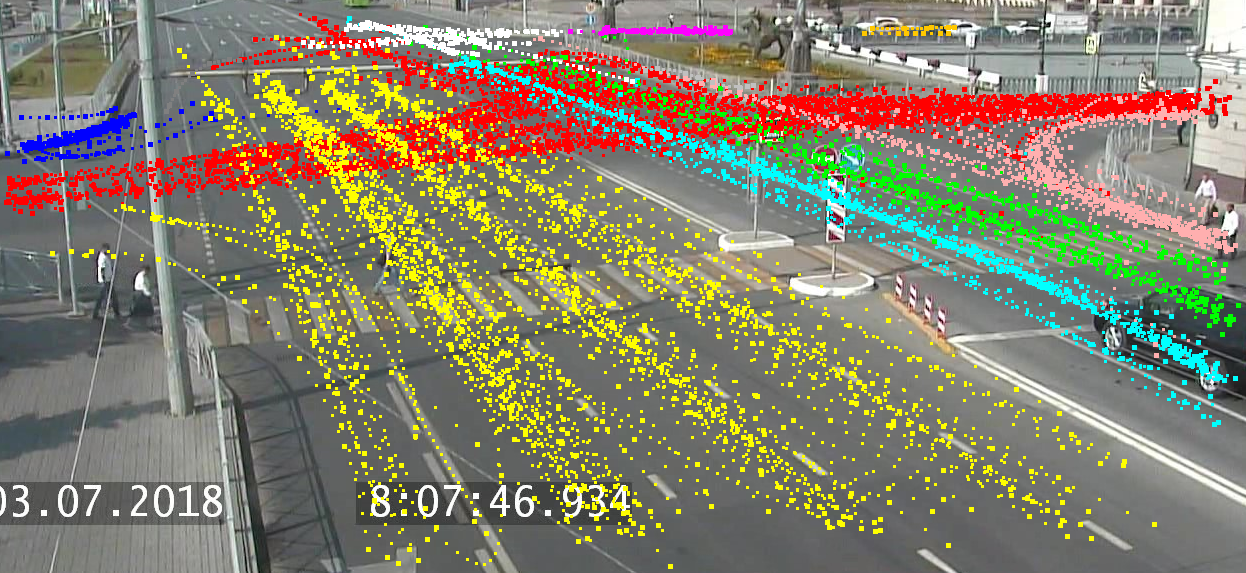
\includegraphics[width=\textwidth]{images/11cl-di-1.jpeg}
		\caption{11 resulting clusters, DI = 0.97}
		\label{fig:11cl-di-1}
	\end{subfigure}
	\hfill
	\begin{subfigure}[!htb]{0.495\textwidth}
		\centering{}
		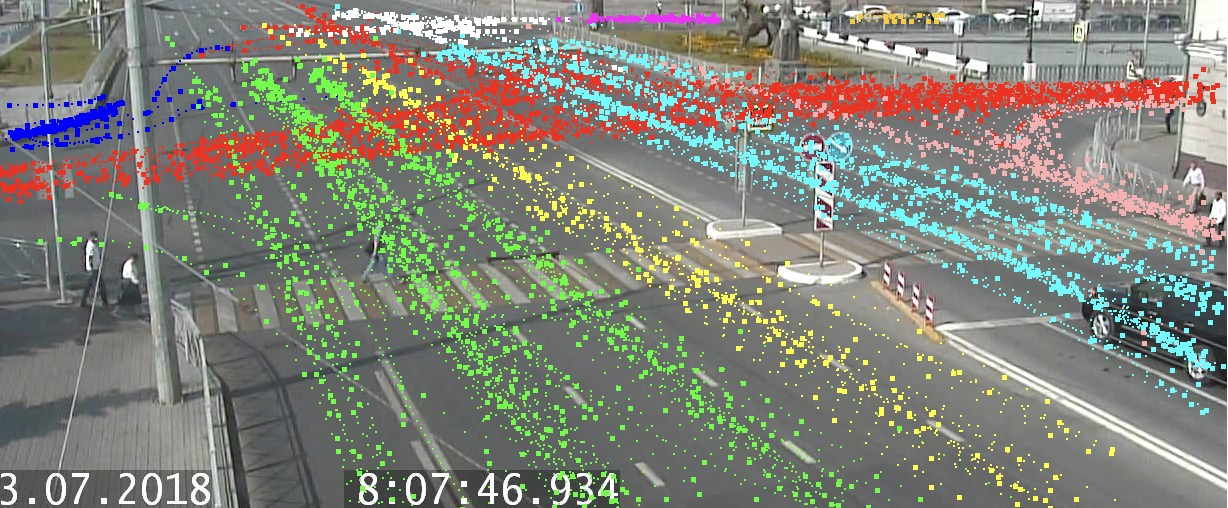
\includegraphics[width=\textwidth]{images/9cl-di-1.jpeg}
		\caption{9 resulting clusters, DI = 0.94}
		\label{fig:9cl-di-1}
	\end{subfigure}
	\hfill
	\begin{subfigure}[!htb]{0.495\textwidth}
		\centering{}
		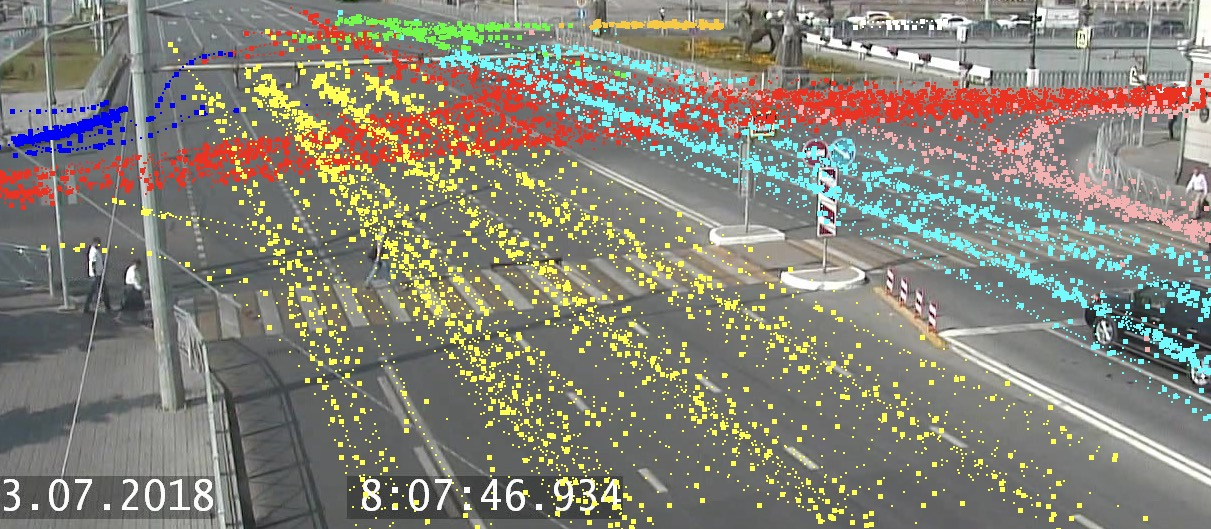
\includegraphics[width=\textwidth]{images/8cl-di-1.jpeg}
		\caption{8 resulting clusters, DI = 0.95}
		\label{fig:8cl-di-1}
	\end{subfigure}
	\hfill
	\begin{subfigure}[!htb]{0.495\textwidth}
		\centering{}
		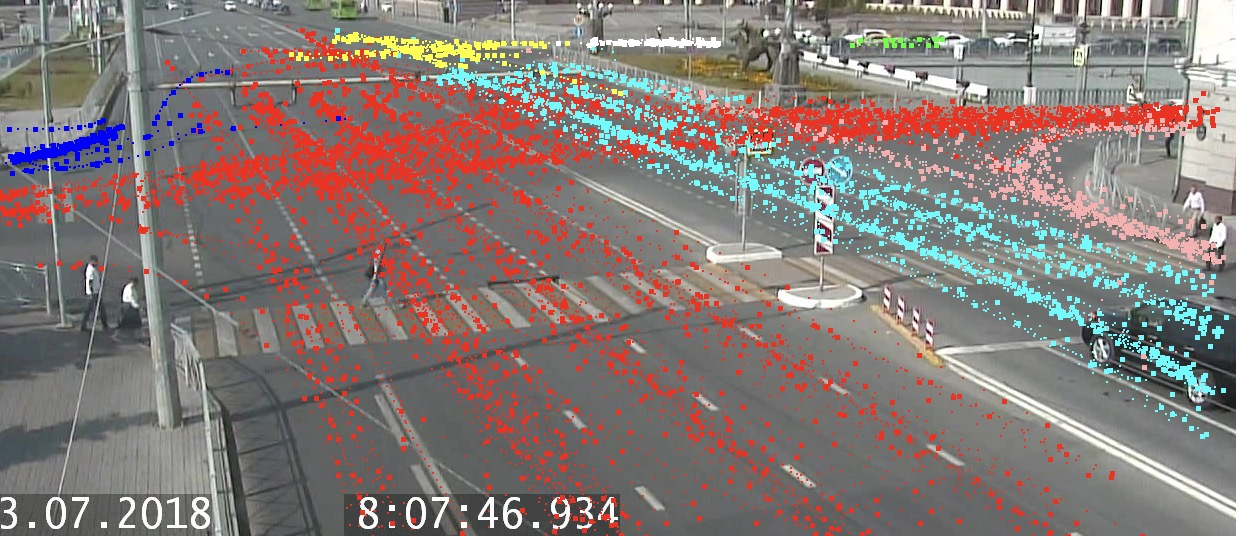
\includegraphics[width=\textwidth]{images/7cl-di-1.jpeg}
		\caption{7 resulting clusters, DI = 0.97}
		\label{fig:7cl-di-1}
	\end{subfigure}
	\caption{Clustering results for adaptive $\bm{\varepsilon}$, $coeff_\varepsilon = 20.0$ ($1.txt$), Polynomial Regression approximation}
	\label{fig:clust-res-1}
\end{figure}

\begin{figure}[!htb]
	\centering
	\begin{subfigure}[!htb]{0.495\textwidth}
		\centering{}
		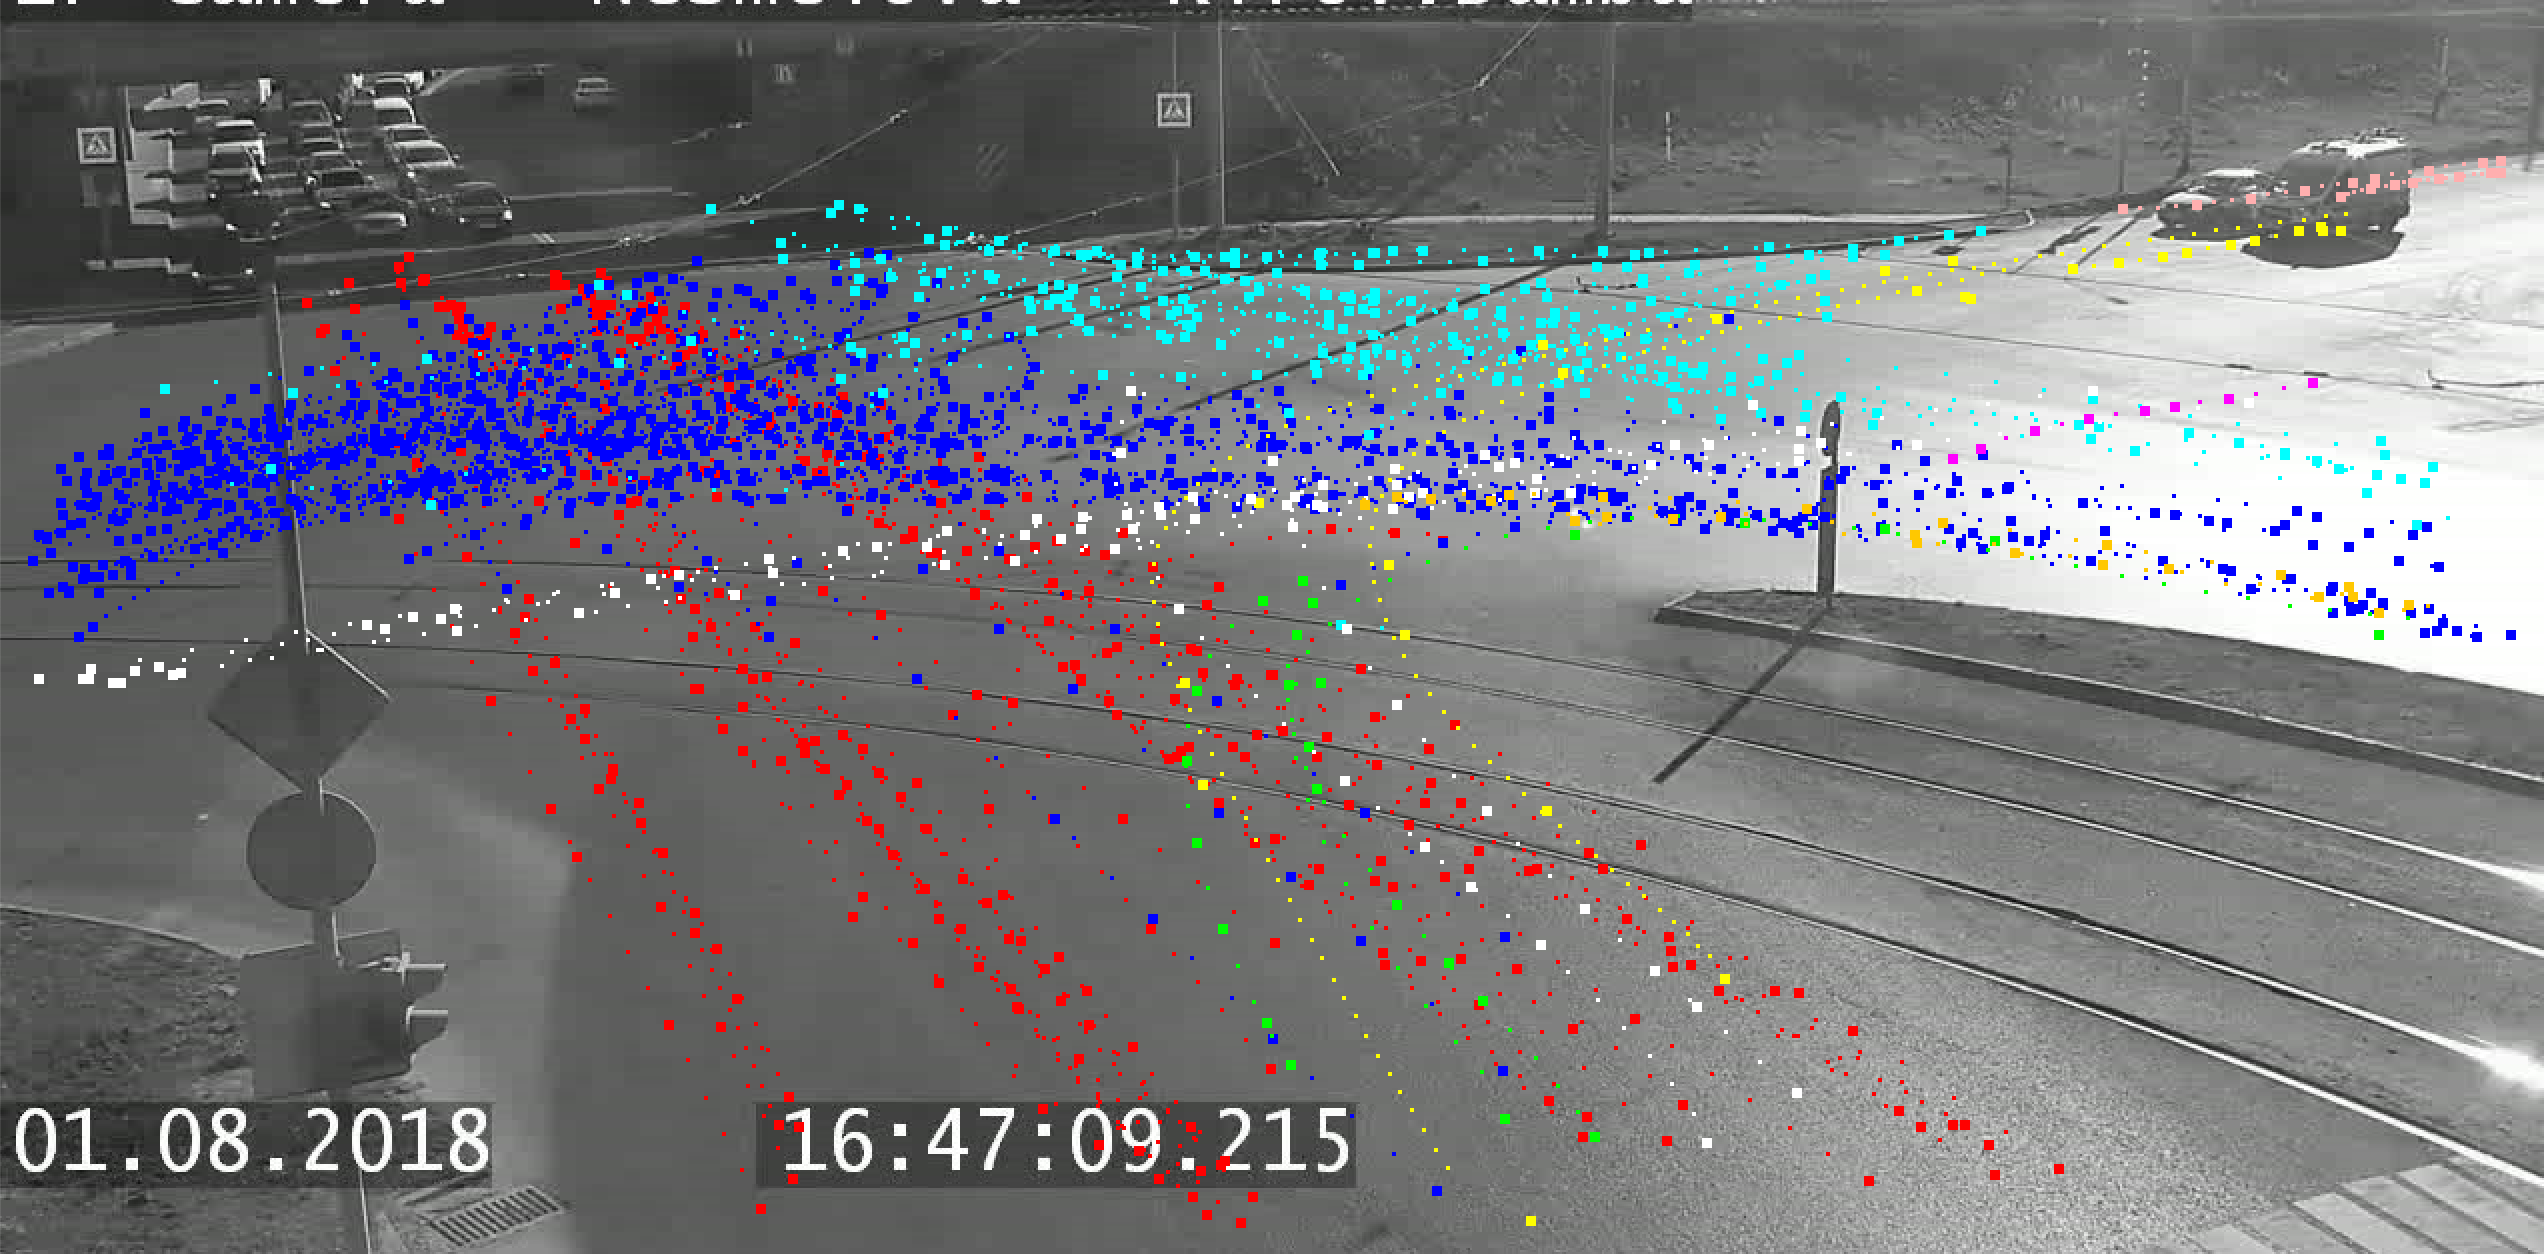
\includegraphics[width=\textwidth]{images/9cl-di-94.png}
		\caption{9 resulting clusters, DI = 0.94}
		\label{fig:9cl-di-94}
	\end{subfigure}
	\hfill
	\begin{subfigure}[!htb]{0.495\textwidth}
		\centering{}
		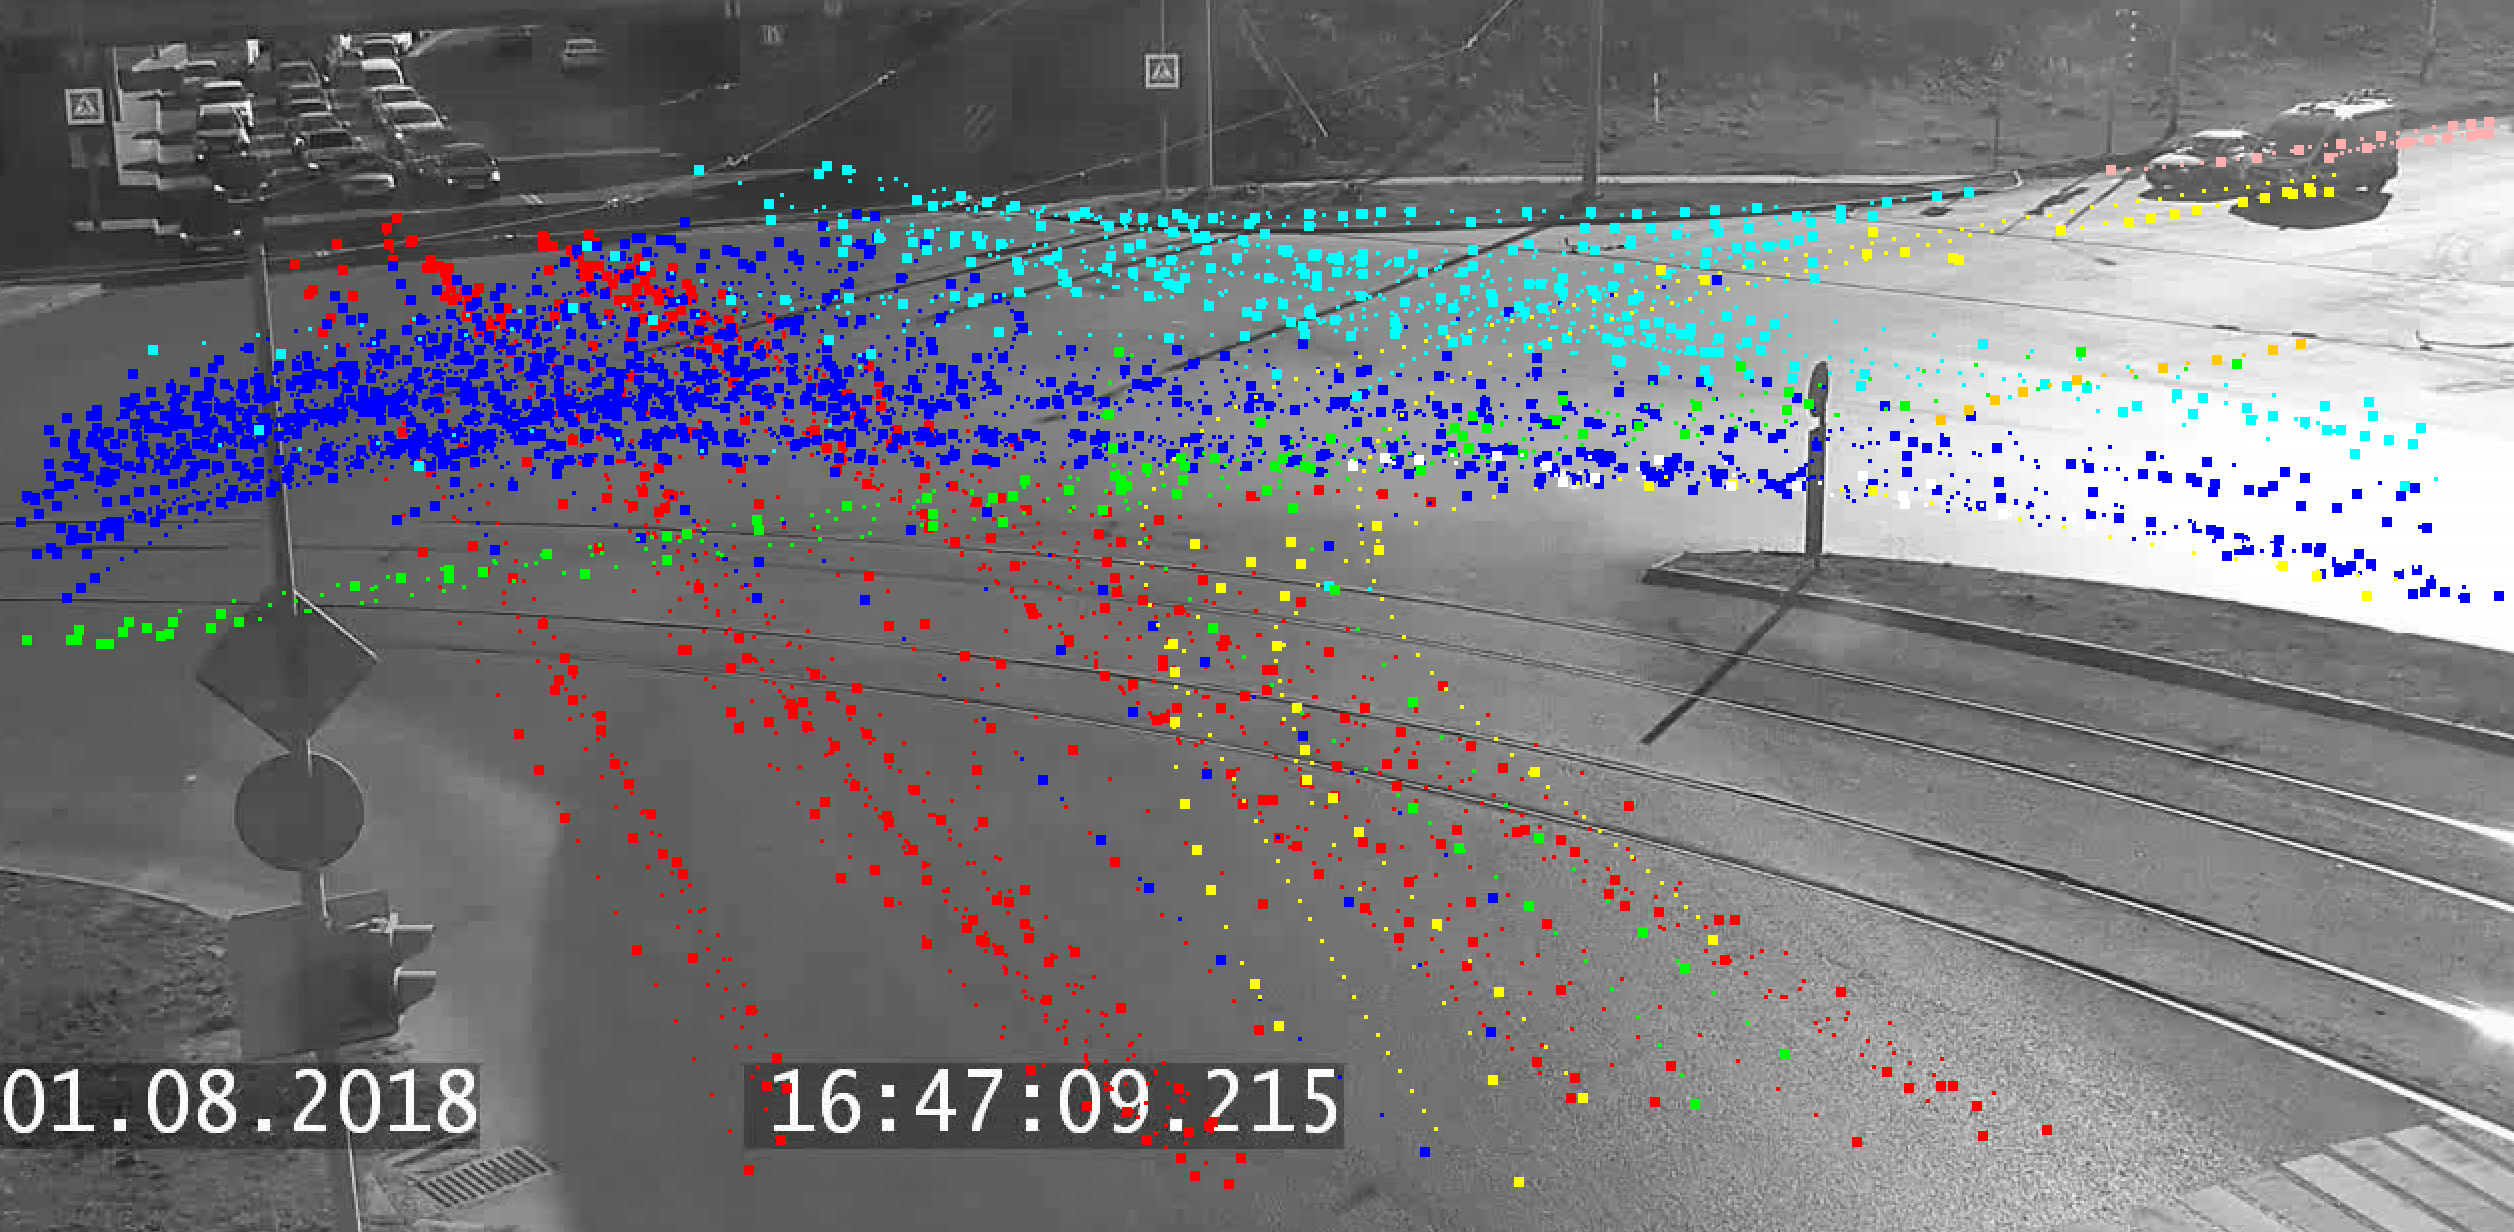
\includegraphics[width=\textwidth]{images/8cl-di-95.png}
		\caption{8 resulting clusters, DI = 0.95}
		\label{fig:8cl-di-95}
	\end{subfigure}
	\hfill
	\begin{subfigure}[!htb]{0.495\textwidth}
		\centering{}
		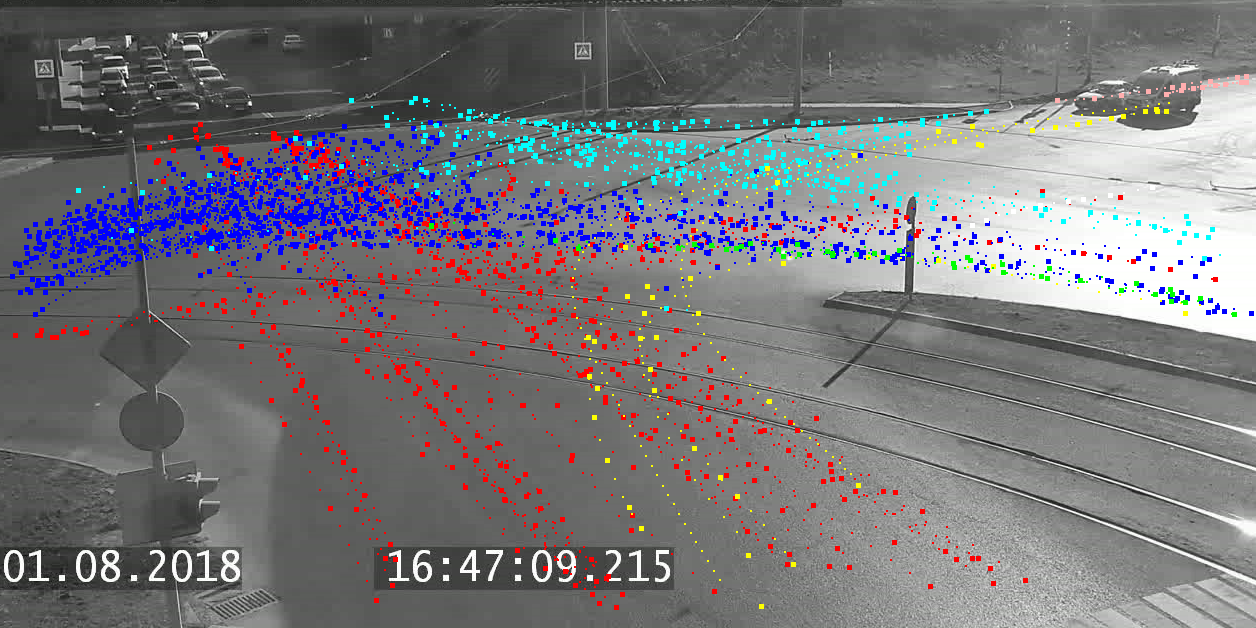
\includegraphics[width=\textwidth]{images/7cl-di-97.png}
		\caption{7 resulting clusters, DI = 0.97}
		\label{fig:7cl-di-97}
	\end{subfigure}
	\caption{Clustering results for adaptive $\bm{\varepsilon}$, $coeff_\varepsilon = 20.0$ ($2.txt$), Polynomial Regression approximation}
	\label{fig:clust-res-2}
\end{figure}

Validation of the resulting clusters was carried out using the DI metric, the following values ​​were obtained:

\begin{itemize}
	\setlength\itemsep{0em}
	\item 9 clusters --> DI = 0.94,
	\item \textbf{8 clusters --> DI = 0.95},
	\item 7 clusters --> DI = 0.97 (visually invalid clusters).
\end{itemize}

However, despite the high DI value, it can be noticed that the clustering result contains errors: blue key points corresponding to the blue cluster of trajectories are superimposed on the trajectories of the red cluster. A possible reason for such a behavior is a high degree of similarity between these trajectories and trajectories from the blue cluster in the upper left half of the figure: this area is represented by a dense accumulation of blue dots.

\subsubsection{Adaptive $\bm{\varepsilon}$ values analysis}

In order to find the best $\varepsilon$ values for each intersection, several experiments were carried out using different $ADAPT\_COEFF_x$ and $ADAPT\_COEFF_y$ values. First experiments were carried out using same coefficient values for both $X$- and $Y$-coordinates, however, for input data from second, third and forth intersections ($2.txt$, $3.txt$, $4.txt$) using different values lead to better results, but not for the first intersection. Also different adaptive parameter value calculation relations were used besides Formulas \ref{eq:epsXY-adapt}. For example, relations from Formula \ref{eq:eps-adapt-1} work better for data from $1.txt$. Using different coefficients also leads to very precise clustering results for all the input files: $ADAPT\_COEFF_x = 15.0$ and $ADAPT\_COEFF_y = 20.0$ (Formula \ref{eq:eps-adapt-234}). Moreover, it was found out that clustering to 11 clusters is more precise than to 7, 8 or 9. Results of clustering are given on Figures \ref{fig:clust-res-1-pr-diff-coeff} -- \ref{fig:clust-res-1-rdp-n-diff-coeff}.

\begin{subequations}\label{eq:eps-adapt-1}
	\begin{align}
		\varepsilon_x = \frac{(maxX - minX)}{\sqrt{distToCP}} \\
		\varepsilon_y = \frac{(maxX - minX)}{\sqrt{distToCP}}
	\end{align}
\end{subequations}

\begin{subequations}\label{eq:eps-adapt-234}
	\begin{align}
		\varepsilon_x = coeff_{\varepsilon}X * \frac{(maxX - minX)}{distToCP}, coeff_{\varepsilon}X = 15.0 \\
		\varepsilon_y = coeff_{\varepsilon}Y * \frac{(maxX - minX)}{distToCP}, coeff_{\varepsilon}Y = 20.0
	\end{align}
\end{subequations}

\begin{figure}[!htb]
	\centering
	\begin{subfigure}[!htb]{0.23\textwidth}
		\centering{}
		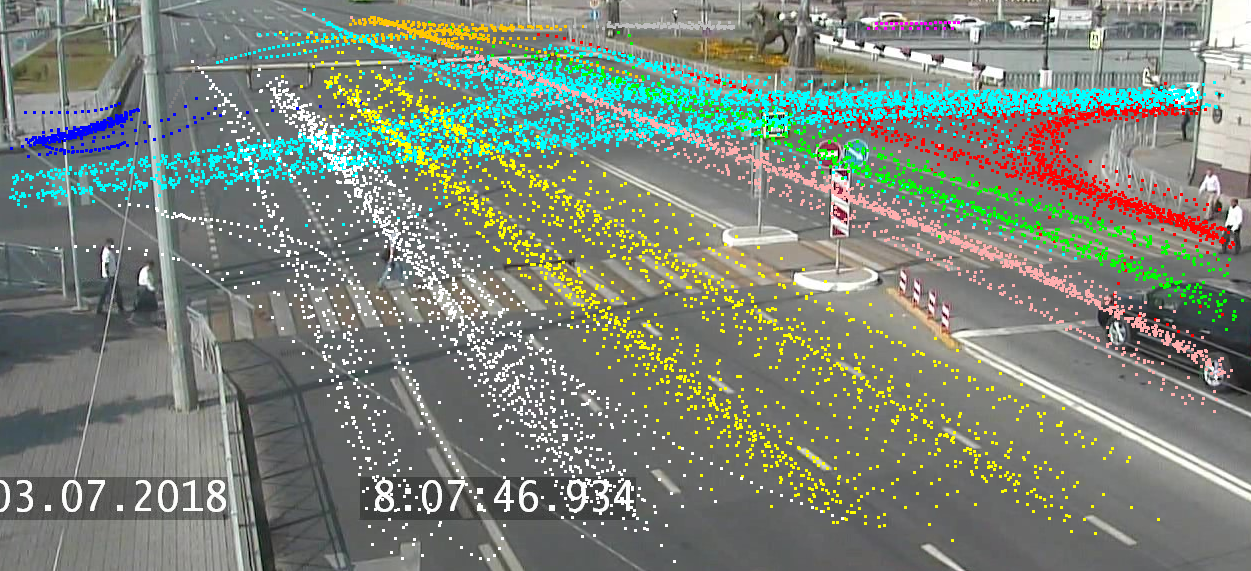
\includegraphics[width=\textwidth]{images/cl-res/clust-res-1-pr-diff-coeff-1.png}
		\caption{11 resulting clusters, DI = 0.97 ($1.txt$)}
		\label{fig:clust-res-1-pr-diff-coeff-1}
	\end{subfigure}
	\hfill
	\begin{subfigure}[!htb]{0.23\textwidth}
		\centering{}
		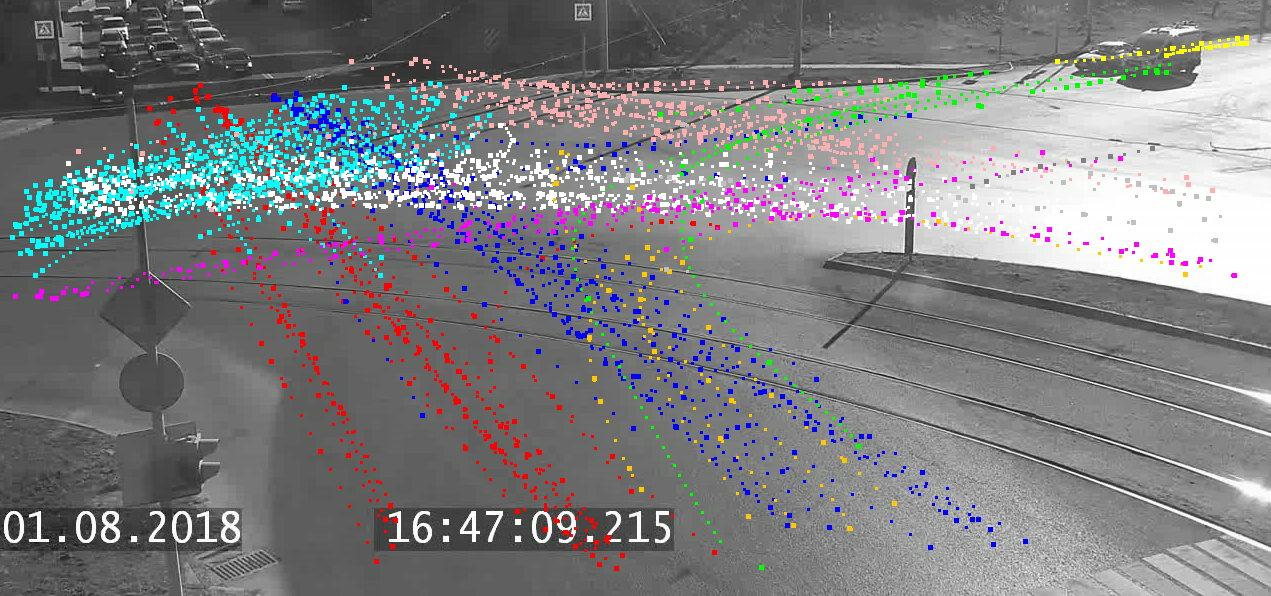
\includegraphics[width=\textwidth]{images/cl-res/clust-res-1-pr-diff-coeff-2.png}
		\caption{11 resulting clusters, DI = 0.94 ($2.txt$)}
		\label{fig:clust-res-1-pr-diff-coeff-2}
	\end{subfigure}
	\hfill
	\begin{subfigure}[!htb]{0.23\textwidth}
		\centering{}
		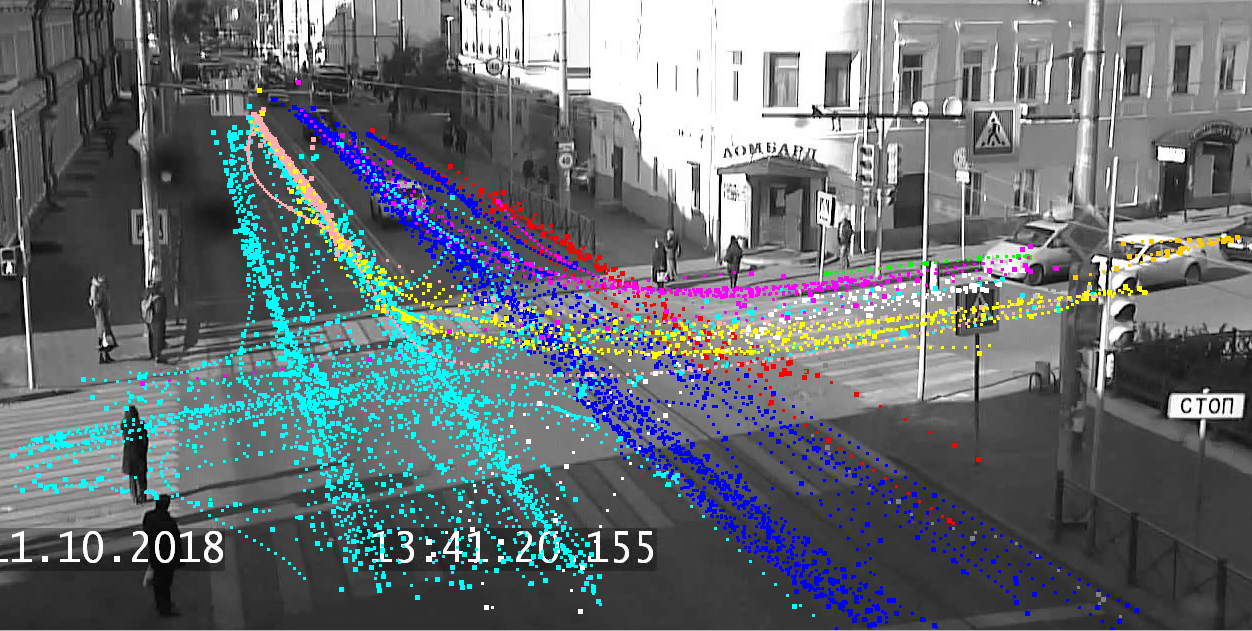
\includegraphics[width=\textwidth]{images/cl-res/clust-res-1-pr-diff-coeff-3.png}
		\caption{11 resulting clusters, DI = 0.90 ($3.txt$)}
		\label{fig:clust-res-1-pr-diff-coeff-3}
	\end{subfigure}
	\hfill
	\begin{subfigure}[!htb]{0.23\textwidth}
		\centering{}
		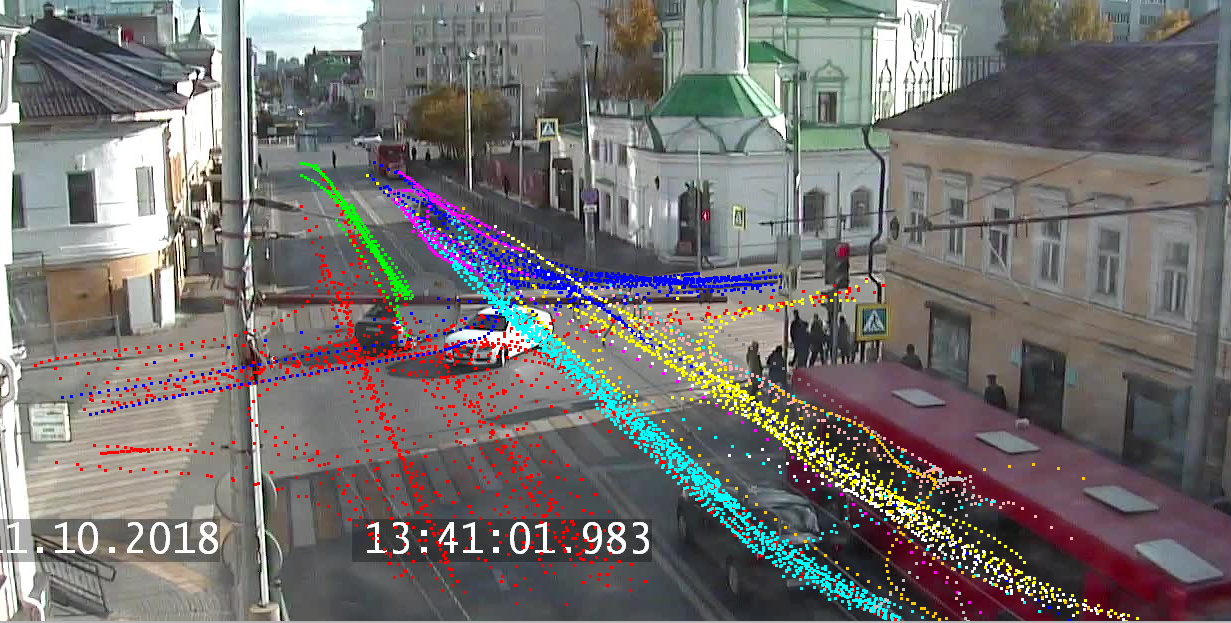
\includegraphics[width=\textwidth]{images/cl-res/clust-res-1-rdp-n-diff-coeff-4.png}
		\caption{11 resulting clusters, DI = 0.91 ($4.txt$)}
		\label{fig:clust-res-1-pr-diff-coeff-4}
	\end{subfigure}
	\caption{Clustering results for adaptive $\bm{\varepsilon}$ using Formula \ref{eq:eps-adapt-234}, Polynomial Regression approximation, $N = 8$}
	\label{fig:clust-res-1-pr-diff-coeff}
\end{figure}

\begin{figure}[!htb]
	\centering
	\begin{subfigure}[!htb]{0.23\textwidth}
		\centering{}
		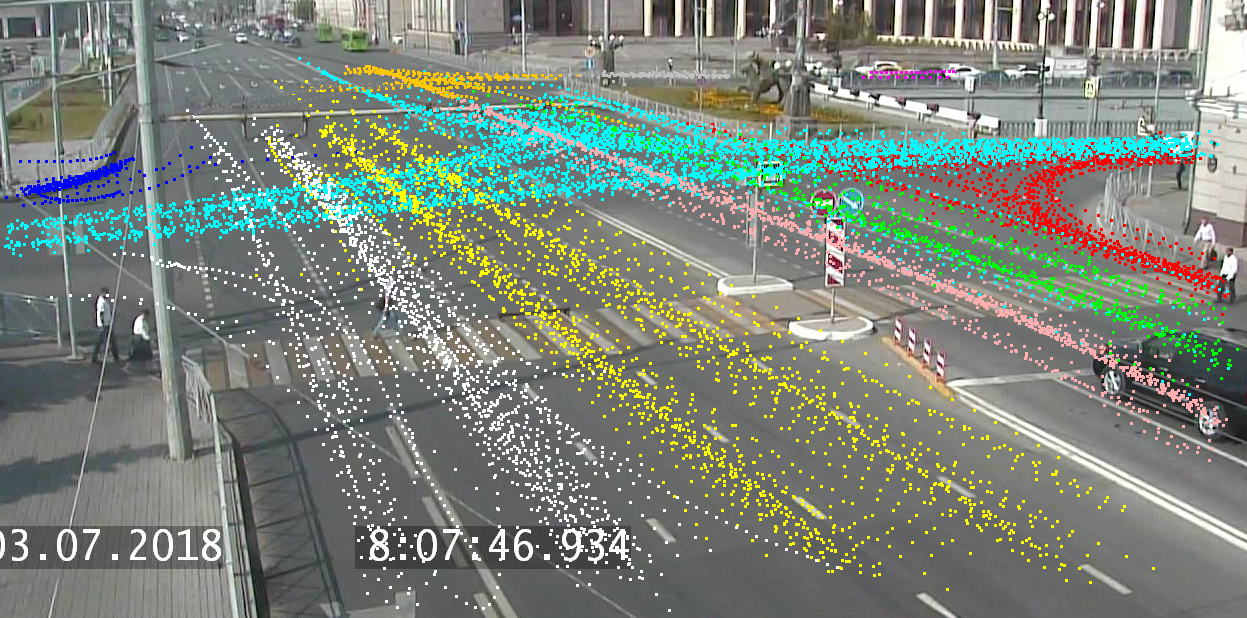
\includegraphics[width=\textwidth]{images/cl-res/clust-res-1-rdp-n-diff-coeff-1.png}
		\caption{11 resulting clusters, DI = 0.97 ($1.txt$)}
		\label{fig:clust-res-1-rdp-n-diff-coeff-1}
	\end{subfigure}
	\hfill
	\begin{subfigure}[!htb]{0.23\textwidth}
		\centering{}
		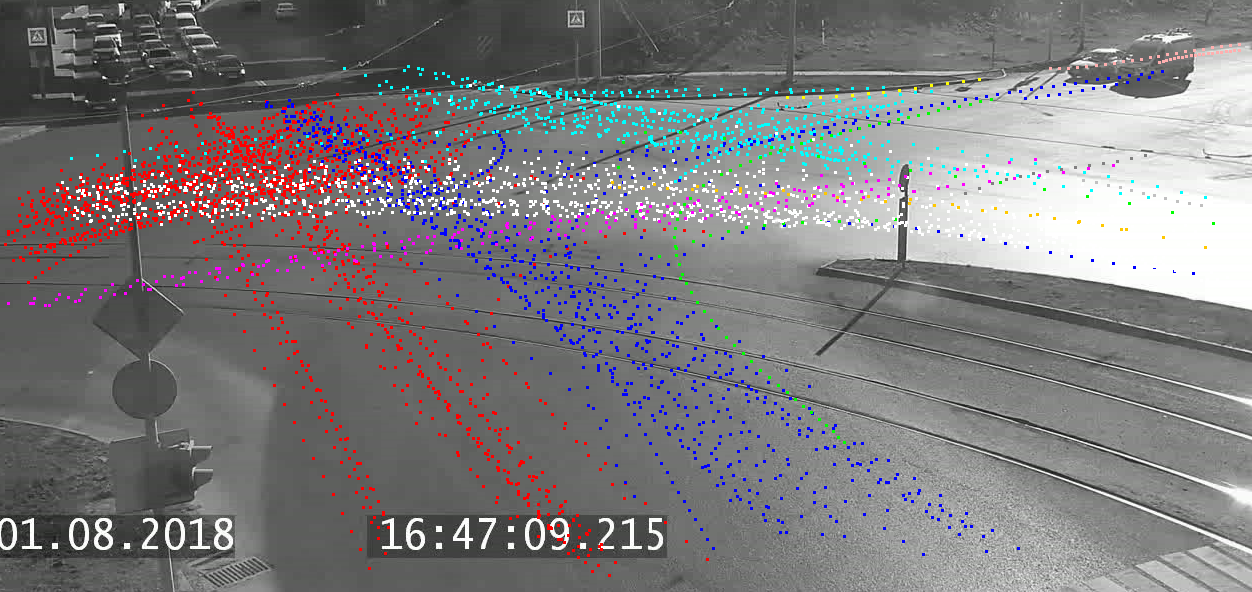
\includegraphics[width=\textwidth]{images/cl-res/clust-res-1-rdp-n-diff-coeff-2.png}
		\caption{11 resulting clusters, DI = 0.95 ($2.txt$)}
		\label{fig:clust-res-1-rdp-n-diff-coeff-2}
	\end{subfigure}
	\hfill
	\begin{subfigure}[!htb]{0.23\textwidth}
		\centering{}
		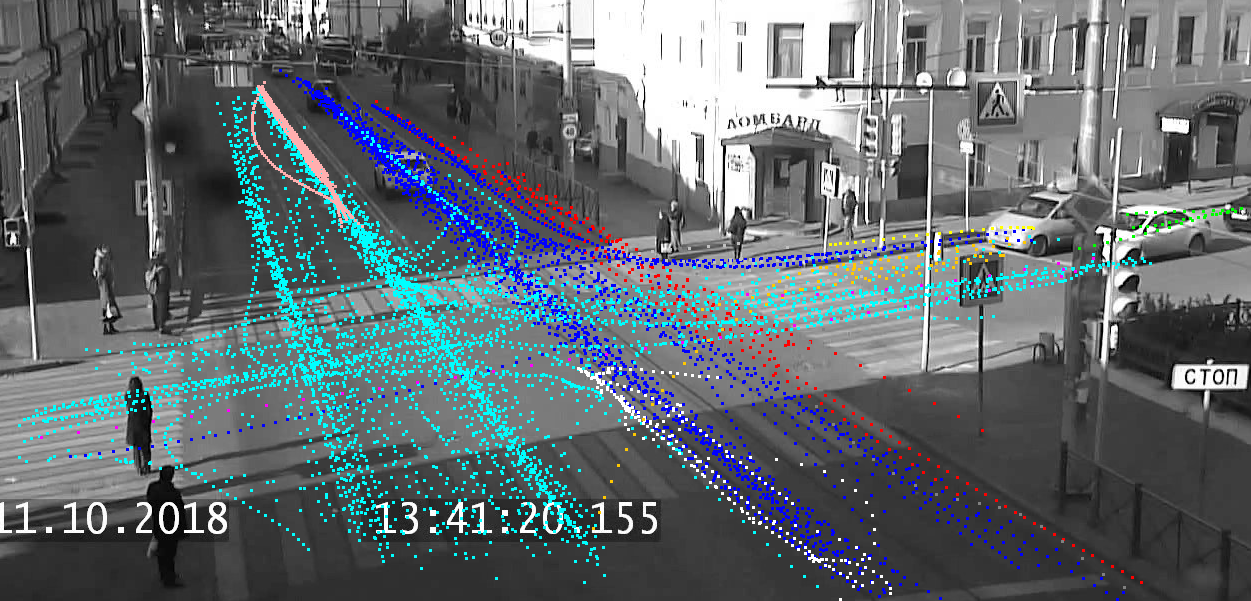
\includegraphics[width=\textwidth]{images/cl-res/clust-res-1-rdp-n-diff-coeff-3.png}
		\caption{11 resulting clusters, DI = 0.93 ($3.txt$)}
		\label{fig:clust-res-1-rdp-n-diff-coeff-3}
	\end{subfigure}
	\hfill
	\begin{subfigure}[!htb]{0.23\textwidth}
		\centering{}
		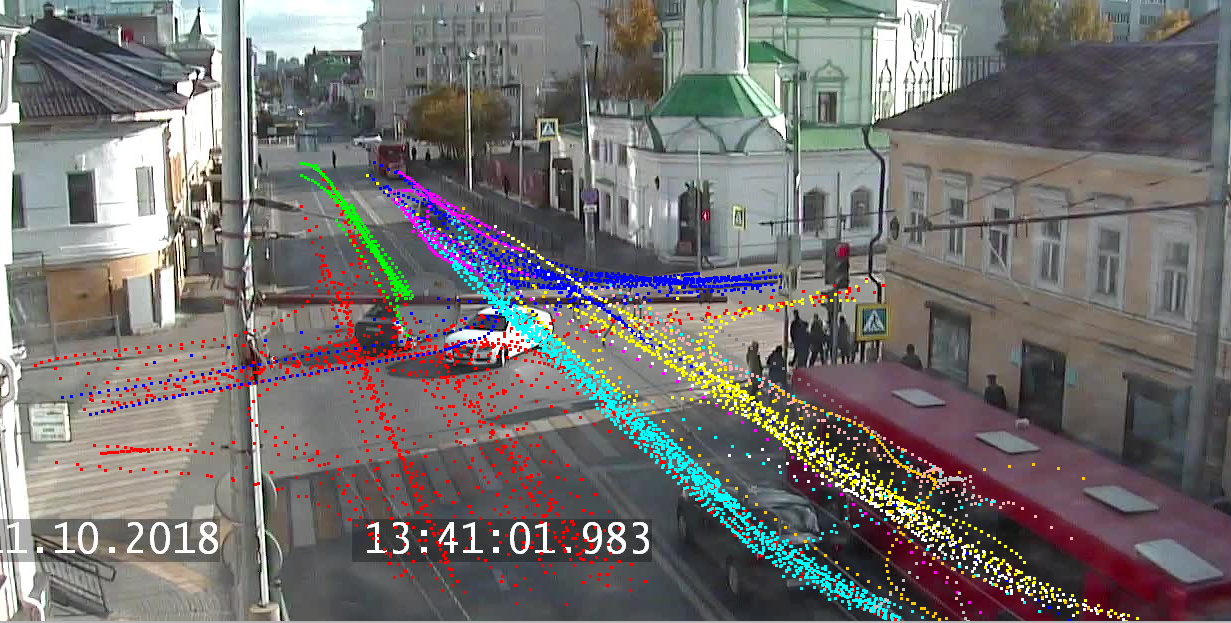
\includegraphics[width=\textwidth]{images/cl-res/clust-res-1-rdp-n-diff-coeff-4.png}
		\caption{11 resulting clusters, DI = 0.92 ($4.txt$)}
		\label{fig:clust-res-1-rdp-n-diff-coeff-4}
	\end{subfigure}
	\caption{Clustering results for adaptive $\bm{\varepsilon}$ using Formula \ref{eq:eps-adapt-234}, Douglas-Peucker N approximation, $N = 8$}
	\label{fig:clust-res-1-rdp-n-diff-coeff}
\end{figure}

Moreover, in order to deal with the extremely huge values of $ADAPT\_COEFF$ parameters which occur close to camera point, following line was added to calculation method to restrict the upper boundary (Formulas \ref{eq:adapt-eps-upper-limit}):

\begin{subequations}\label{eq:adapt-eps-upper-limit}
	\begin{align}
		\varepsilon_x = cpDist < 250\ ?\ 250 : \varepsilon_x \\
		\varepsilon_y = cpDist < 250\ ?\ 250 : \varepsilon_y
	\end{align}
\end{subequations}

However experiments showed that using different upper boundaries for different files works better. For example data from $2.txt$, $3.txt$ and $4.txt$ is being clustered better while using different values (Formula \ref{eq:adapt-eps-upper-limit-new}):

\begin{subequations}\label{eq:adapt-eps-upper-limit-new}
	\begin{align}
	\varepsilon_x = cpDist < 250\ ?\ 250 : \varepsilon_x \\
	\varepsilon_y = cpDist < 150\ ?\ 200 : \varepsilon_y
	\end{align}
\end{subequations}

Result of clustering using equations from Formula \ref{eq:adapt-eps-upper-limit-new} is given in Figure \ref{fig:clust-res-1-regr-sqrt}.

\begin{figure}[!htb]
	\centering
	\begin{subfigure}[!htb]{0.23\textwidth}
		\centering{}
		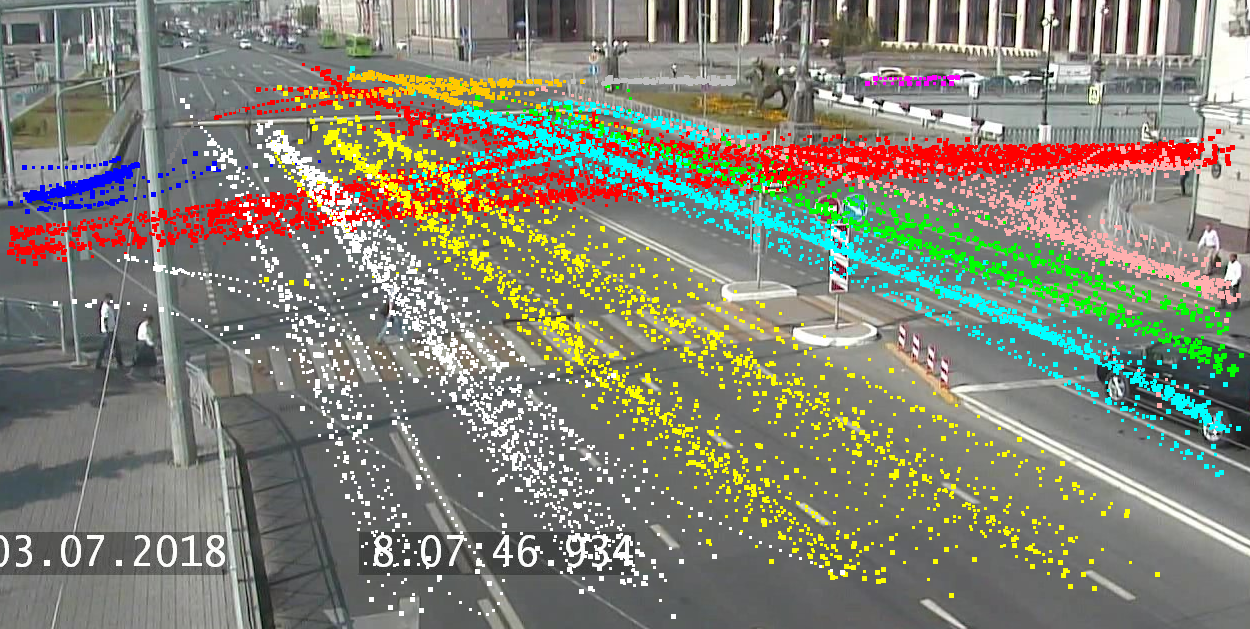
\includegraphics[width=\textwidth]{images/cl-res/clust-res-1-regr-sqrt-1.png}
		\caption{11 resulting clusters, DI = 0.94 ($1.txt$)}
		\label{fig:clust-res-1-regr-sqrt-1}
	\end{subfigure}
	\hfill
	\begin{subfigure}[!htb]{0.23\textwidth}
		\centering{}
		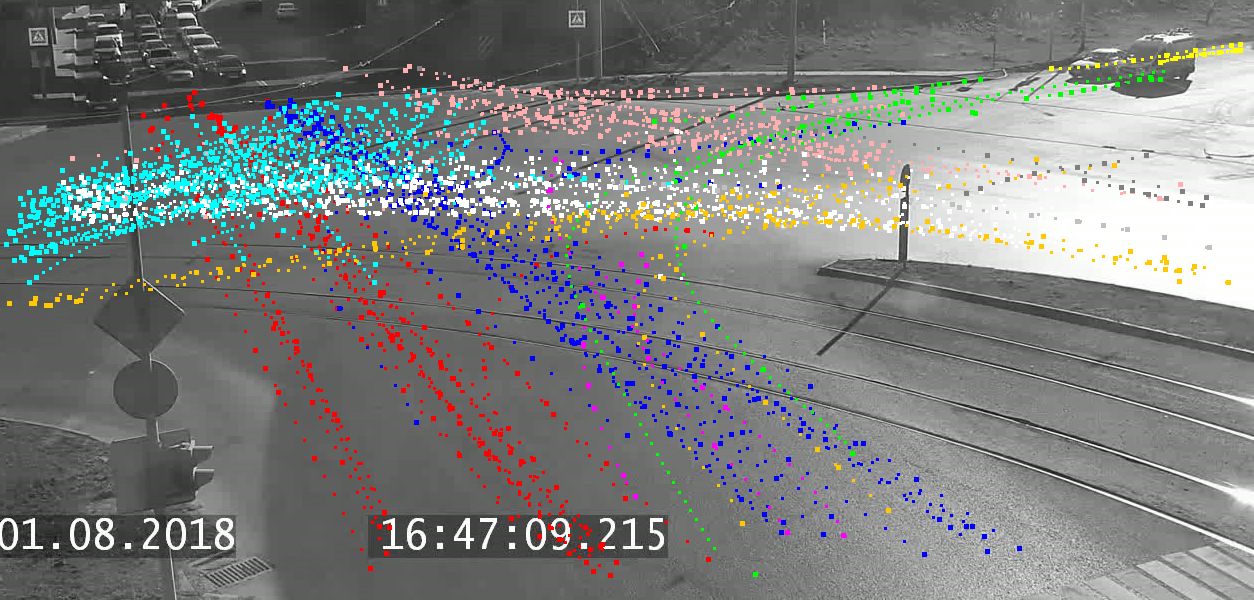
\includegraphics[width=\textwidth]{images/cl-res/clust-res-1-regr-sqrt-2.png}
		\caption{9 resulting clusters, DI = 0.93 ($2.txt$)}
		\label{fig:clust-res-1-regr-sqrt-2}
	\end{subfigure}
	\hfill
	\begin{subfigure}[!htb]{0.23\textwidth}
		\centering{}
		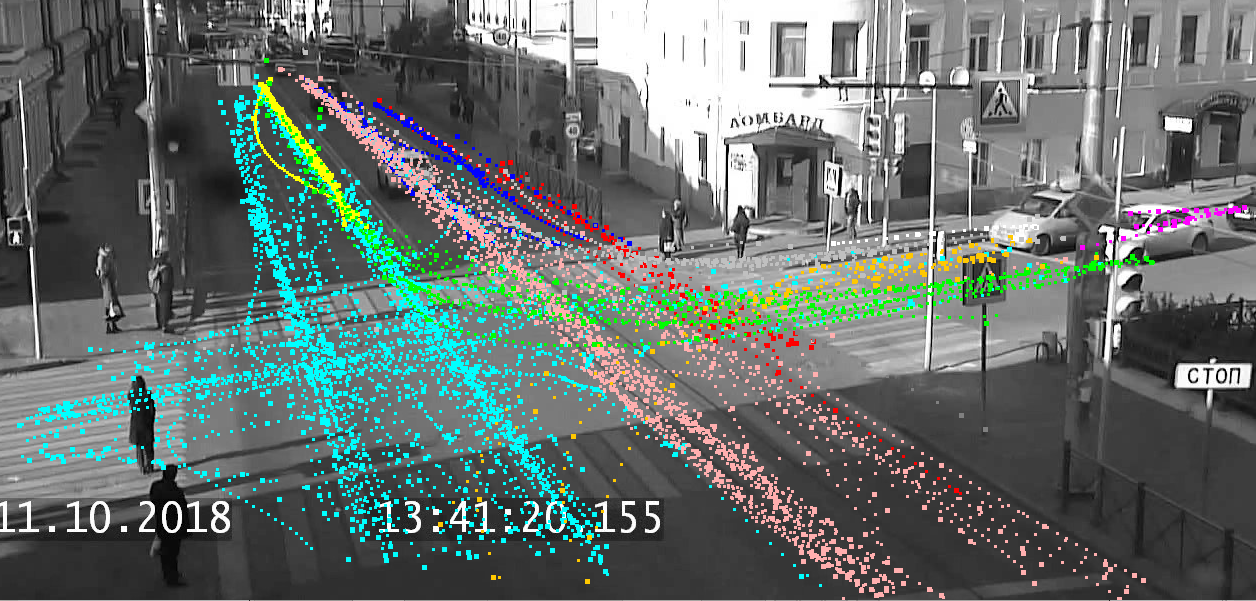
\includegraphics[width=\textwidth]{images/cl-res/clust-res-1-regr-sqrt-3.png}
		\caption{8 resulting clusters, DI = 0.87 ($3.txt$)}
		\label{fig:clust-res-1-regr-sqrt-3}
	\end{subfigure}
	\hfill
	\begin{subfigure}[!htb]{0.23\textwidth}
		\centering{}
		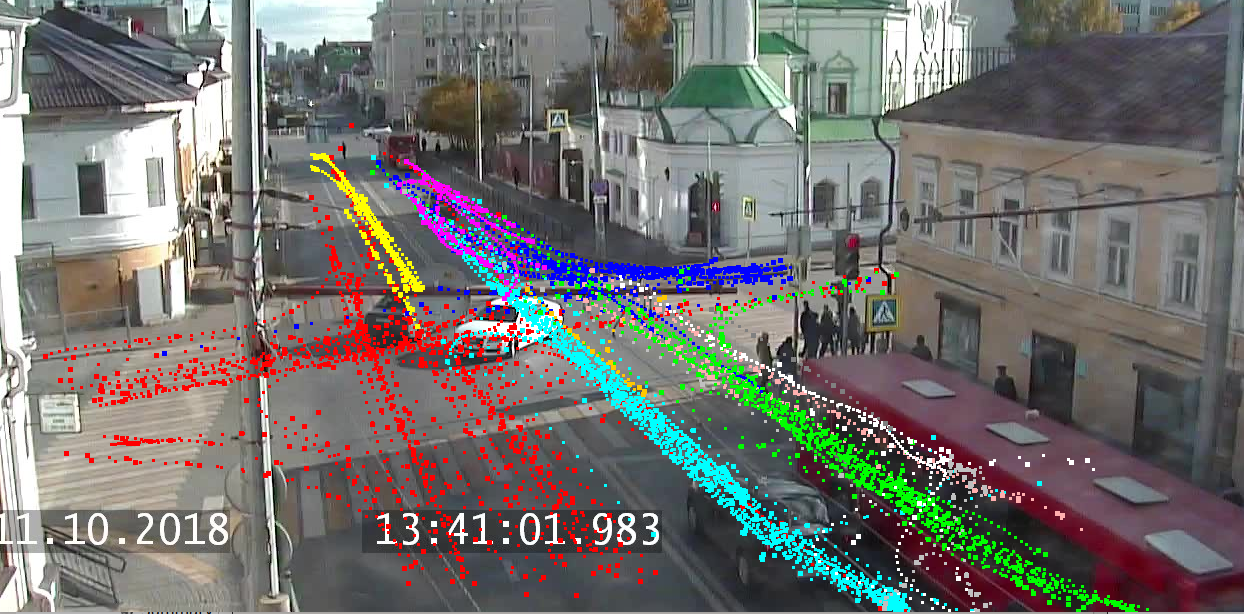
\includegraphics[width=\textwidth]{images/cl-res/clust-res-1-regr-sqrt-4.png}
		\caption{7 resulting clusters, DI = 0.87 ($4.txt$)}
		\label{fig:clust-res-1-regr-sqrt-4}
	\end{subfigure}
	\caption{Clustering results for adaptive $\bm{\varepsilon}$ from Formula \ref{eq:eps-adapt-1} with limits from Formula \ref{eq:adapt-eps-upper-limit-new}, Polynomial Regression approximation}
	\label{fig:clust-res-1-regr-sqrt}
\end{figure}

\subsubsection{Approximation Methods Comparison}

Clustering was performed and evaluated using filtered trajectories approximated by both Polynomial Regression and Douglas-Peucker N algorithms. Results of clustering using an adaptive $\varepsilon$ with the $adapt\_coeff = 20.0$ are presented on Figure \ref{fig:clust-res-1-rdp-n}.

\begin{figure}[!htb]
	\centering
	\begin{subfigure}[!htb]{0.495\textwidth}
		\centering{}
		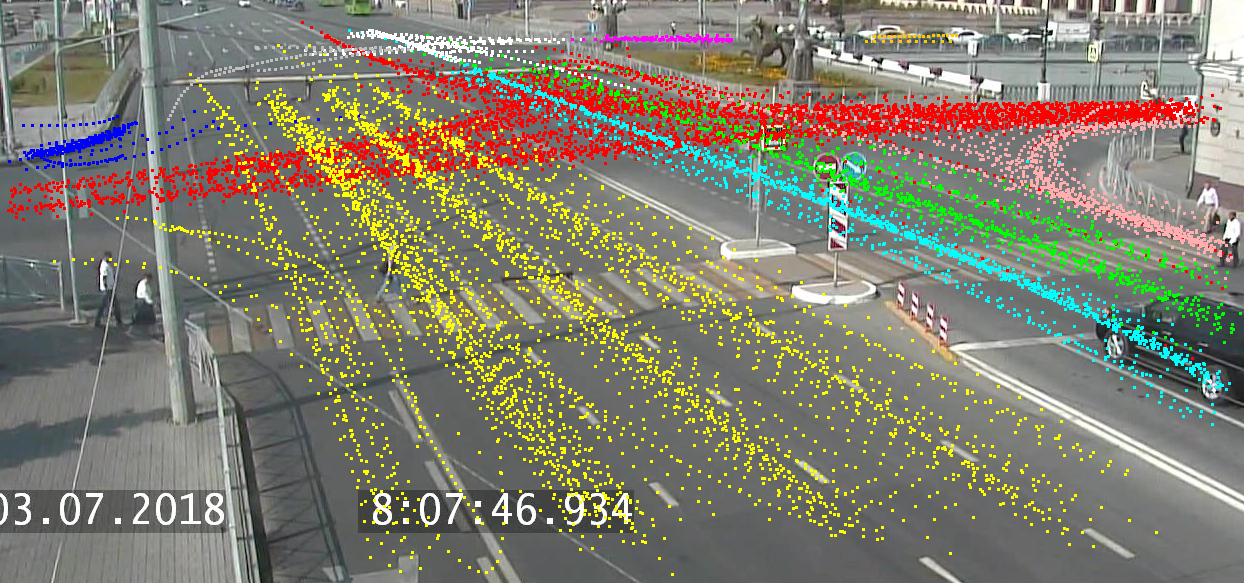
\includegraphics[width=\textwidth]{images/10cl-rdp-n-1.png}
		\caption{10 resulting clusters, DI = 0.97}
		\label{fig:10cl-rdp-n-1}
	\end{subfigure}
	\hfill
	\begin{subfigure}[!htb]{0.495\textwidth}
		\centering{}
		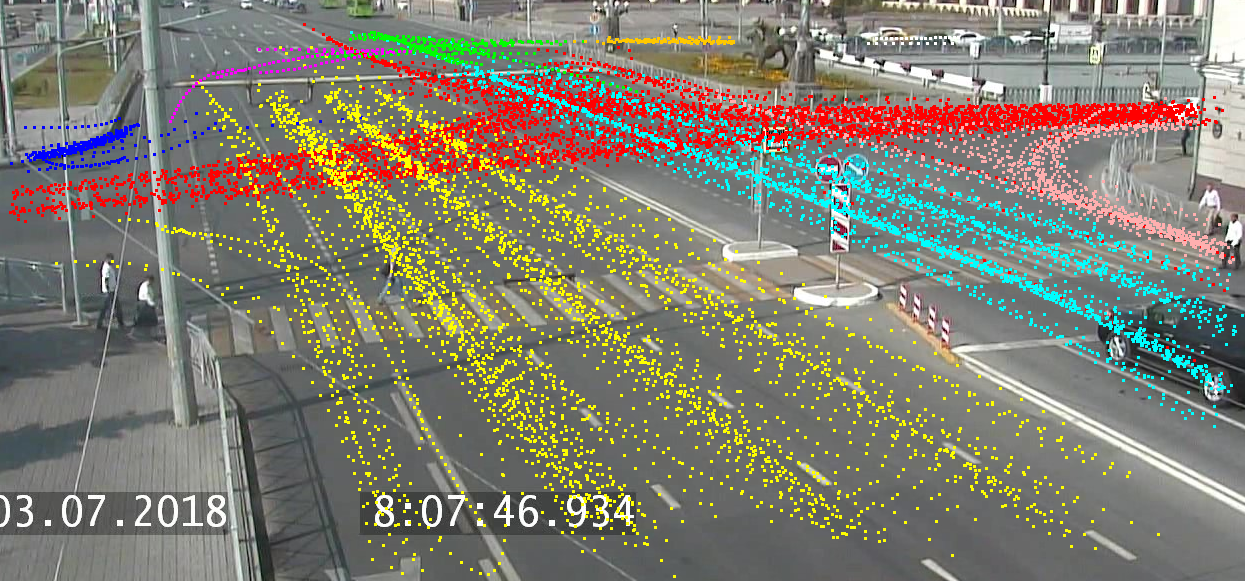
\includegraphics[width=\textwidth]{images/9cl-rdp-n-1.png}
		\caption{9 resulting clusters, DI = 0.97}
		\label{fig:9cl-rdp-n-1}
	\end{subfigure}
	\hfill
	\begin{subfigure}[!htb]{0.495\textwidth}
		\centering{}
		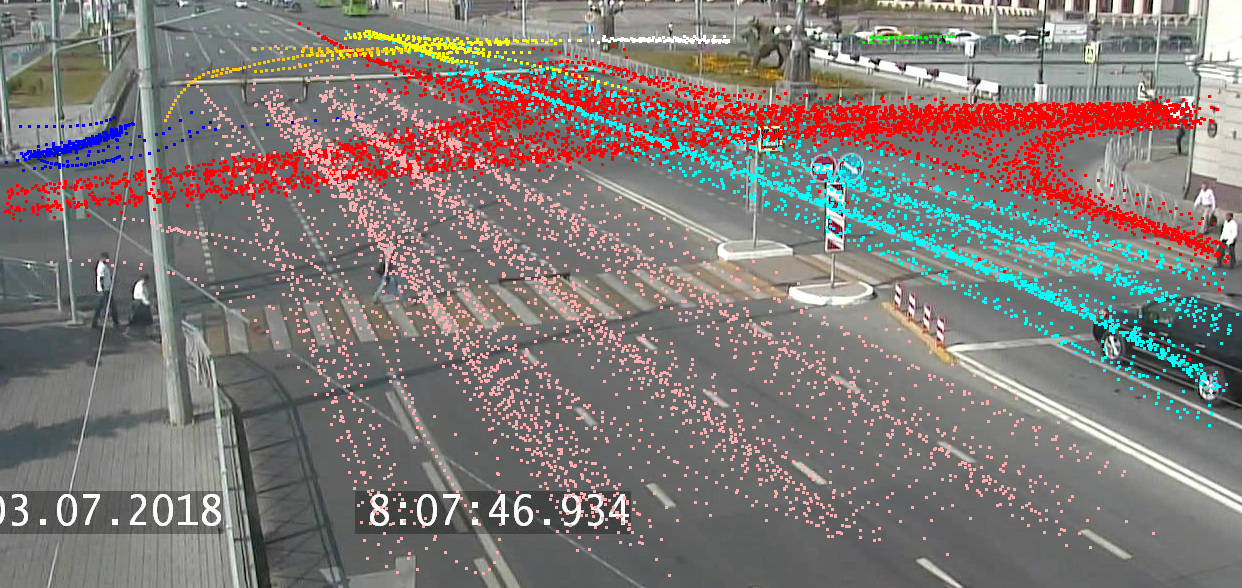
\includegraphics[width=\textwidth]{images/8cl-rdp-n-1.png}
		\caption{8 resulting clusters, DI = 0.98}
		\label{fig:8cl-rdp-n-1}
	\end{subfigure}
	\hfill
	\begin{subfigure}[!htb]{0.495\textwidth}
		\centering{}
		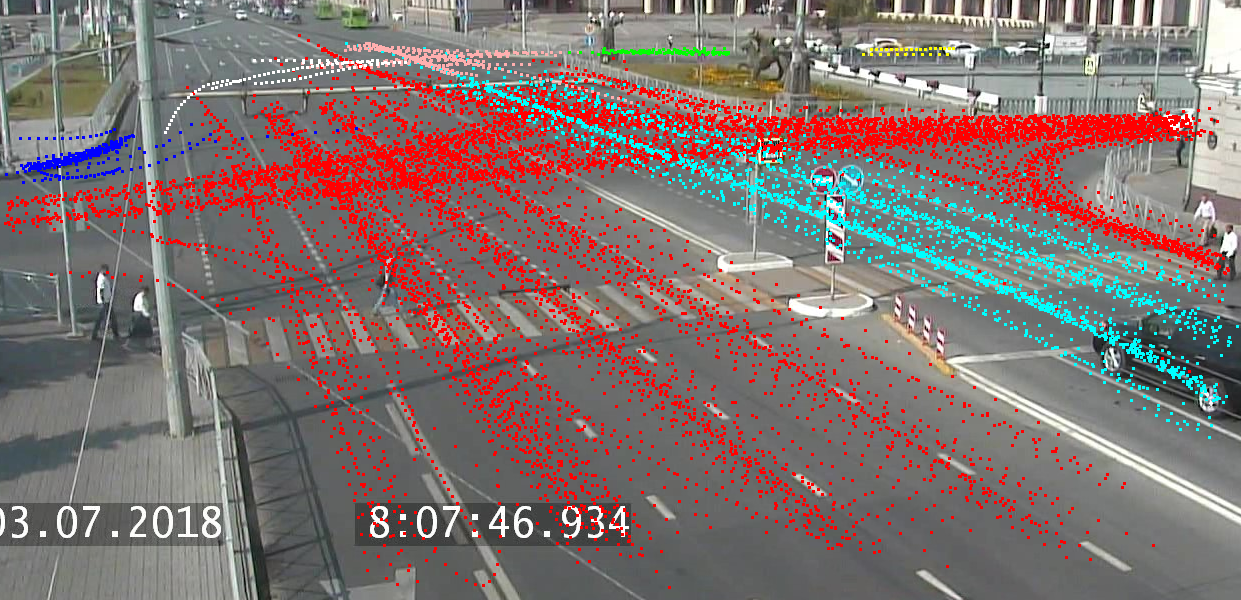
\includegraphics[width=\textwidth]{images/7cl-rdp-n-1.png}
		\caption{7 resulting clusters, DI = 0.99}
		\label{fig:7cl-rdp-n-1}
	\end{subfigure}
	\caption{Clustering results for adaptive $\bm{\varepsilon}$, $coeff_\varepsilon = 20.0$ ($1.txt$), Douglas-Peucker N approximation, $N = 8$}
	\label{fig:clust-res-1-rdp-n}
\end{figure}

As it can be seen from the comparison of Figures \ref{fig:clust-res-1} and \ref{fig:clust-res-1-rdp-n}, clustering the trajectories after Douglas-Peucker N approximation gives more precise results. While considering the images with 9 resulting clusters, in the second case algorithm specified a distinct cluster for the trajectories on the upper part of image related to vehicles with turning trajectories, while in the first case these trajectories were incorrectly included into a red cluster.

\subsubsection{Linkage Methods Comparison}

Different types of linkage methods, which are used in clustering to calculate between-clusters distance, were described in details in previous chapters. According to the tests performed by authors in \cite{inproceedings:7_related_work}, the single linkage method showed the best results and, in view of this, was chosen as a linkage method in the current work. However, evaluations were performed using all three linkage methods in application to used data, and comparison  revealed that average or complete linkage methods demonstrate much more accurate results than single linkage method (Figures \ref{fig:link-meth-comp-stat} -- \ref{fig:link-meth-comp-adapt}). Clustering with single linkage method ends up with almost all trajectories merged into one enormous cluster.

In this section all the results were obtained using trajectories, approximated by Polynomial regression method.

\begin{figure}[!htb]
	\centering
	\begin{subfigure}[!htb]{0.3\textwidth}
		\centering{}
		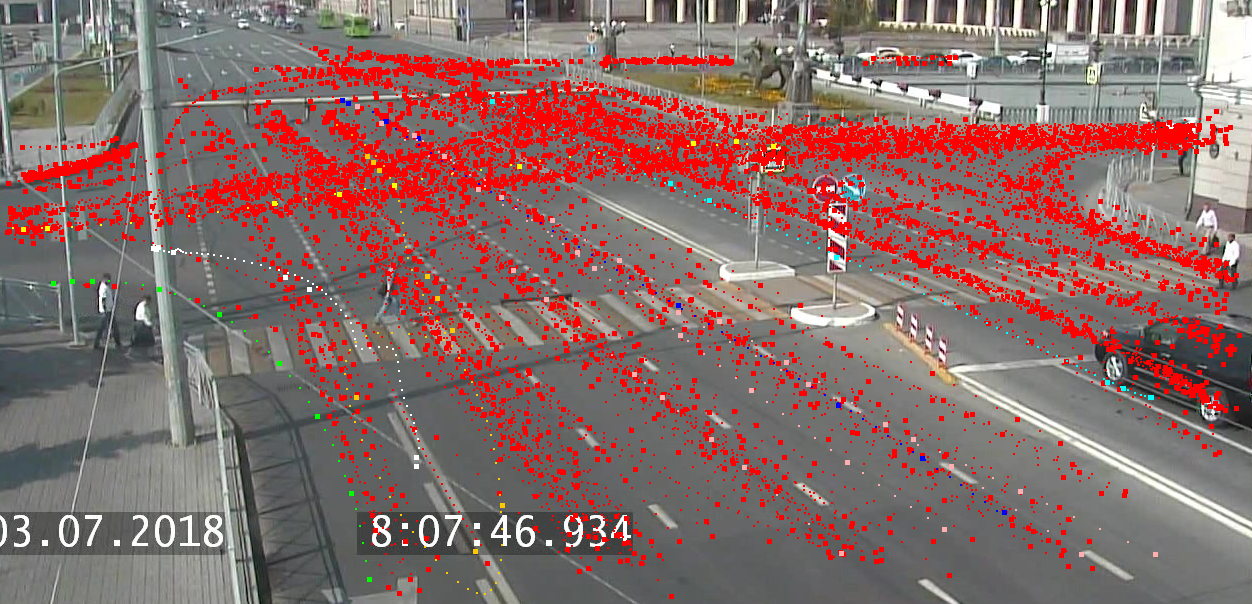
\includegraphics[width=\textwidth]{images/link_meth_comp_stat_min.png}
		\caption{single linkage method, DI = 0.14}
		\label{fig:link-meth-comp-stat-min}
	\end{subfigure}
	\hfill
	\begin{subfigure}[!htb]{0.3\textwidth}
		\centering{}
		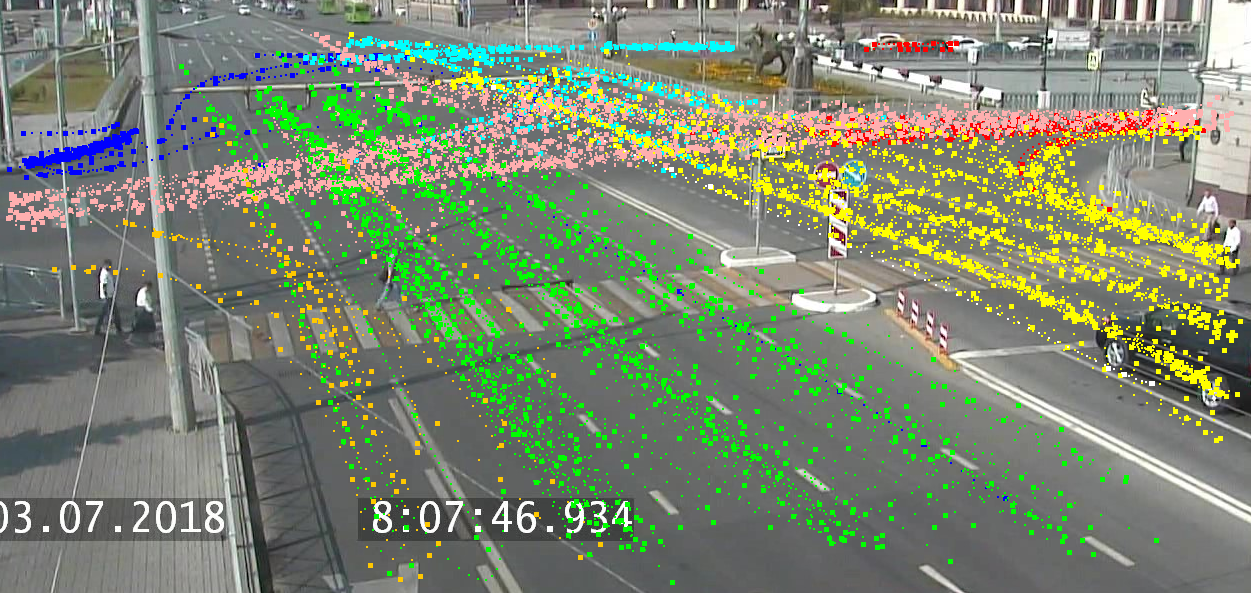
\includegraphics[width=\textwidth]{images/link_meth_comp_stat_avg.png}
		\caption{average linkage method, DI = 0.63}
		\label{fig:link-meth-comp-stat-avg}
	\end{subfigure}
	\hfill
	\begin{subfigure}[!htb]{0.3\textwidth}
		\centering{}
		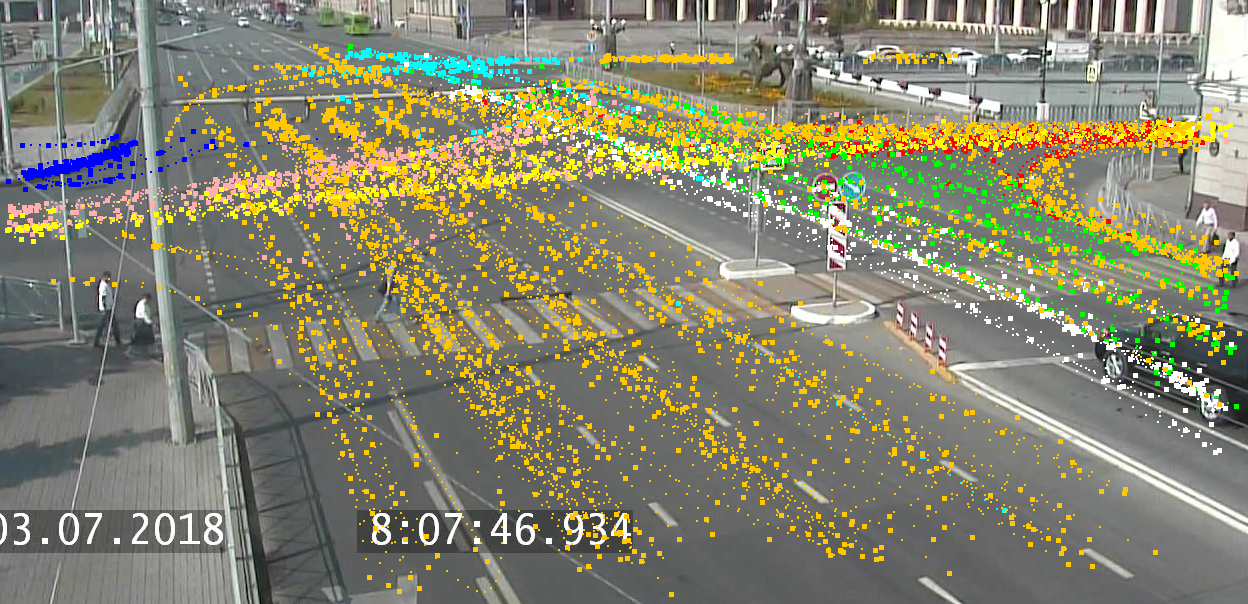
\includegraphics[width=\textwidth]{images/link_meth_comp_stat_max.png}
		\caption{complete linkage method, DI = ~1.0}
		\label{fig:link-meth-comp-stat-max}
	\end{subfigure}
	\caption{Comparison of clusters for different linkage methods, static $\varepsilon = 0.15$ ($1.txt$)}
	\label{fig:link-meth-comp-stat}
\end{figure}

\begin{figure}[!htb]
	\centering
	\begin{subfigure}[!htb]{0.3\textwidth}
		\centering{}
		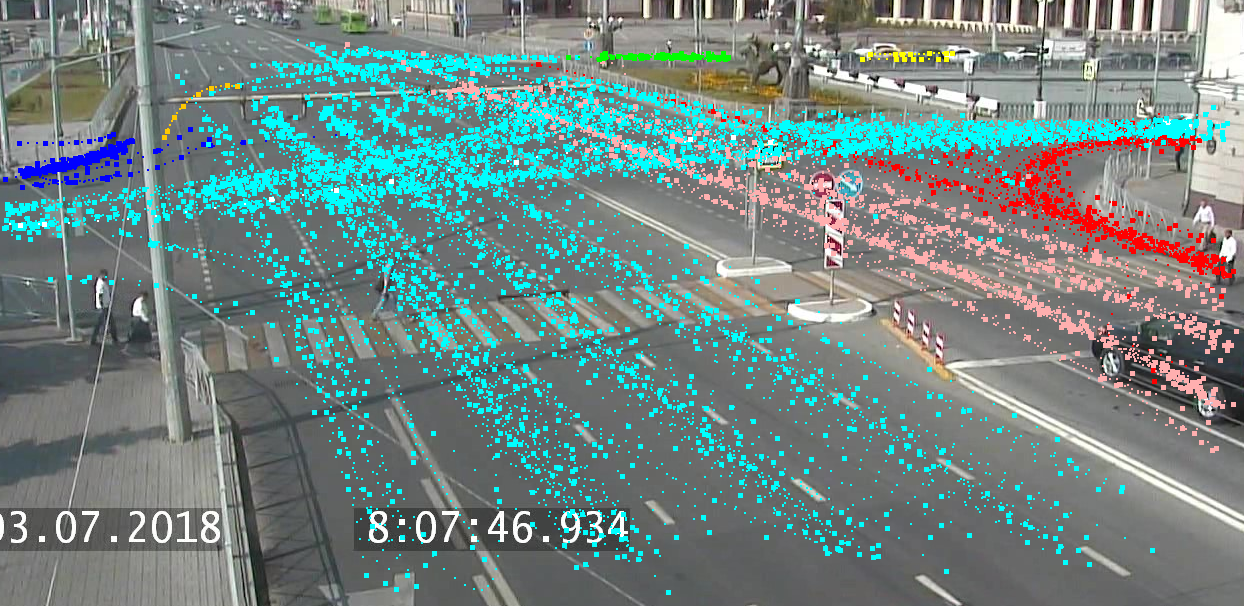
\includegraphics[width=\textwidth]{images/link_meth_comp_adapt_min.png}
		\caption{single linkage method, DI = 0.57}
		\label{fig:link-meth-comp-adapt-min}
	\end{subfigure}
	\hfill
	\begin{subfigure}[!htb]{0.3\textwidth}
		\centering{}
		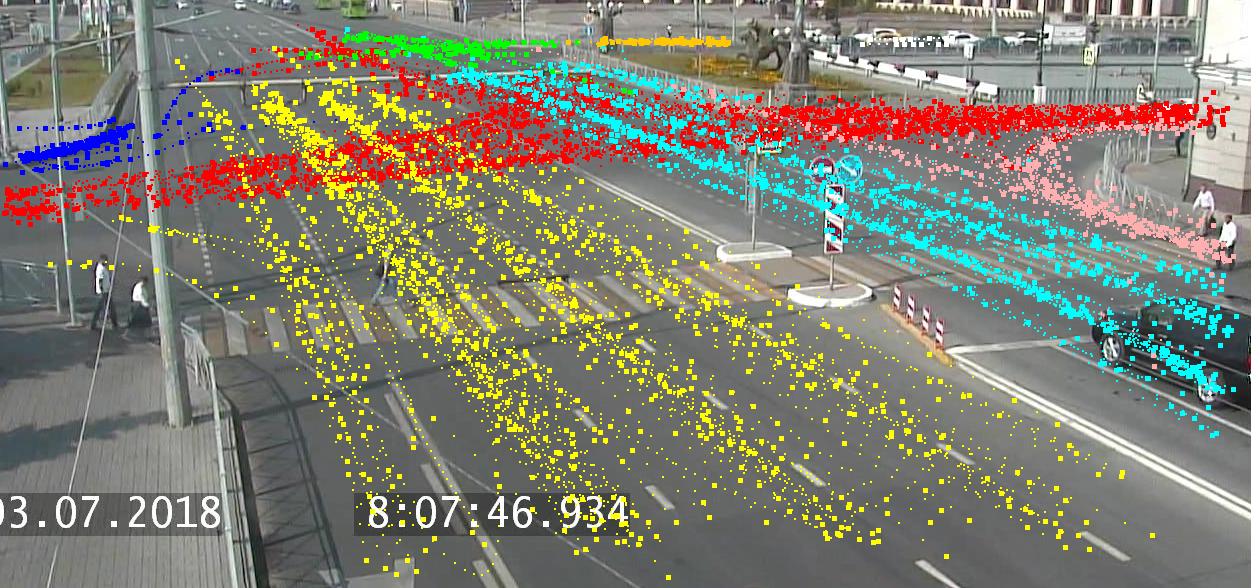
\includegraphics[width=\textwidth]{images/link_meth_comp_adapt_avg.png}
		\caption{average linkage method, DI = 0.97}
		\label{fig:link-meth-comp-adapt-avg}
	\end{subfigure}
	\hfill
	\begin{subfigure}[!htb]{0.3\textwidth}
		\centering{}
		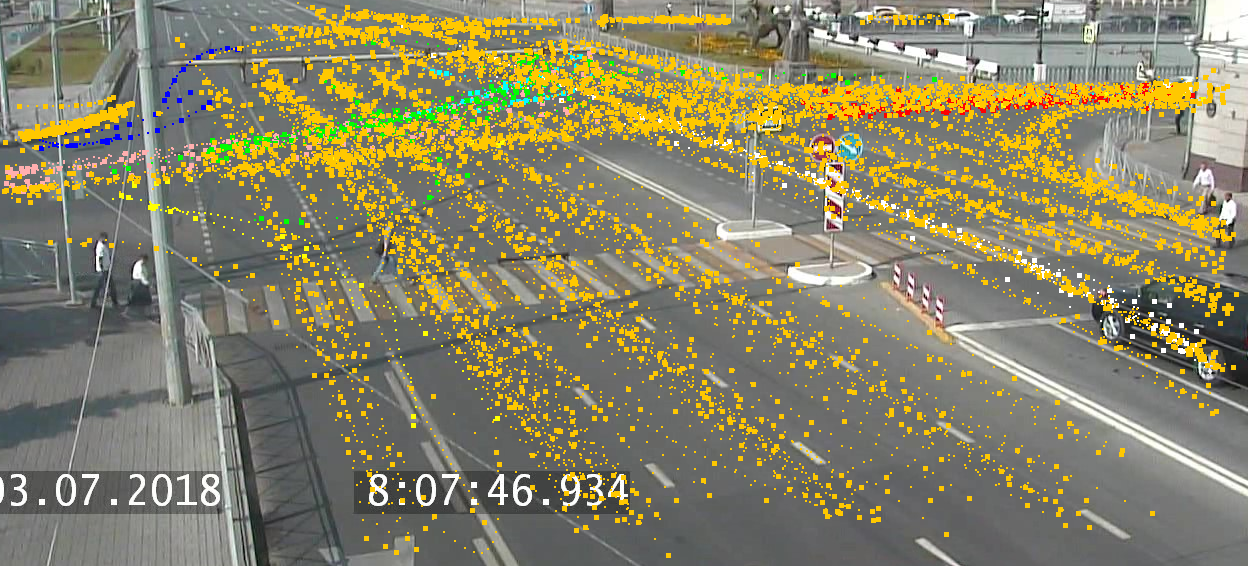
\includegraphics[width=\textwidth]{images/link_meth_comp_adapt_max.png}
		\caption{complete linkage method, DI = ~1.0}
		\label{fig:link-meth-comp-adapt-max}
	\end{subfigure}
	\caption{Comparison of clusters for different linkage methods, static $\varepsilon = 0.15$ ($1.txt$)}
	\label{fig:link-meth-comp-adapt}
\end{figure}

\subsubsection{Summary}

From the above it follows that based on the results of both the quantitative assessment of the DI metric and the visual test resulting clusters are more accurate when clustering till distributing data across 8 clusters for data from both intersections. In other words, 7 clusters are not enough to describe the vehicle trajectory patterns at these intersections. However, when using the static $\varepsilon$ parameter, clustering is more accurate for 9 clusters for data from both intersections.

Moreover, according to the results, the use of adaptive values for the $\varepsilon$ parameter improved the clustering results significantly.

\subsection{Clusters Classification Results}

As it was described in the previous chapter, clusters with small cardinalities are considered as clusters of anomalous trajectories. Figures \ref{fig:cl-classif-res-1} -- \ref{fig:cl-classif-res-2} depict normal and anomalous clusters for data from first and second intersections respectfully.

\begin{figure}[!htb]
	\centering
	\begin{subfigure}[!htb]{0.495\textwidth}
		\centering{}
		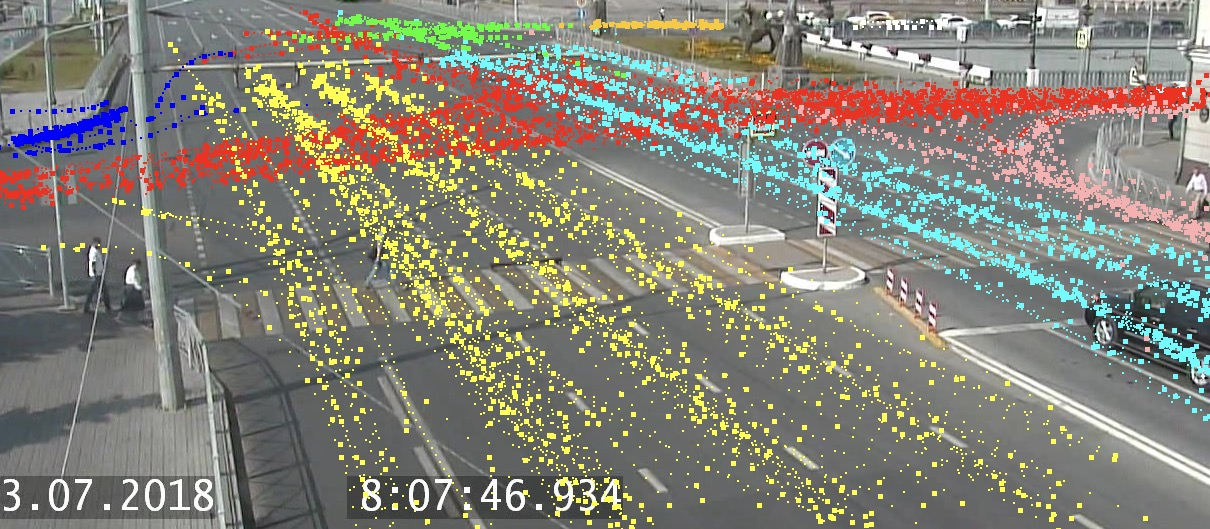
\includegraphics[width=\textwidth]{images/cl-classif-norm-1.jpeg}
		\caption{all clusters (8 clusters)}
		\label{fig:cl-classif-norm-1}
	\end{subfigure}
	\hfill
	\begin{subfigure}[!htb]{0.495\textwidth}
		\centering{}
		\includegraphics[width=\textwidth]{images/cl-classif-anom-1.jpeg}
		\caption{anomalous clusters}
		\label{fig:cl-classif-anom-1}
	\end{subfigure}
	\hfill
	\begin{subfigure}[!htb]{0.495\textwidth}
		\centering{}
		\includegraphics[width=\textwidth]{images/cl-classif-norm-11.png}
		\caption{all clusters (11 clusters, different $\varepsilon$ coefficients)}
		\label{fig:cl-classif-norm-11}
	\end{subfigure}
	\hfill
	\begin{subfigure}[!htb]{0.495\textwidth}
		\centering{}
		\includegraphics[width=\textwidth]{images/cl-classif-anom-11.png}
		\caption{anomalous clusters}
		\label{fig:cl-classif-anom-11}
	\end{subfigure}
	\caption{Normal and anomalous clusters classification results ($1.txt$)}
	\label{fig:cl-classif-res-1}
\end{figure}

\begin{figure}[!htb]
	\centering
	\begin{subfigure}[!htb]{0.495\textwidth}
		\centering{}
		\includegraphics[width=\textwidth]{images/cl-classif-norm-2.jpeg}
		\caption{all clusters}
		\label{fig:cl-classif-norm-2}
	\end{subfigure}
	\hfill
	\begin{subfigure}[!htb]{0.495\textwidth}
		\centering{}
		\includegraphics[width=\textwidth]{images/cl-classif-anom-2.jpeg}
		\caption{anomalous clusters}
		\label{fig:cl-classif-anom-2}
	\end{subfigure}
	\caption{Normal and anomalous clusters classification results ($2.txt$)}
	\label{fig:cl-classif-res-2}
\end{figure}

\subsection{Trajectories Classification Results}


Figures \ref{fig:classif-norm-res-1} -- \ref{fig:classif-norm-res-2} present the classification results using normal trajectories. Red trajectories denote the closest cluster; blue trajectory, depicted using bold \textit{TPs}, emphasizes the corresponding \textit{CM}; the input trajectory plotted using cyan color.

\begin{figure}[!htb]
	\centering
	\begin{subfigure}[!htb]{0.40\textwidth}
		\centering{}
		\includegraphics[width=\textwidth]{images/classif-res/classif-norm-res-1-1.jpeg}
		\caption{}
	\end{subfigure}
	\hfill
	\begin{subfigure}[!htb]{0.57\textwidth}
		\centering{}
		\includegraphics[width=\textwidth]{images/classif-res/classif-norm-res-1-2.jpeg}
		\caption{}
	\end{subfigure}
	\hfill
	\begin{subfigure}[!htb]{0.485\textwidth}
		\centering{}
		\includegraphics[width=\textwidth]{images/classif-res/classif-norm-res-1-3.jpeg}
		\caption{}
	\end{subfigure}
	\hfill
	\begin{subfigure}[!htb]{0.485\textwidth}
		\centering{}
		\includegraphics[width=\textwidth]{images/classif-res/classif-norm-res-1-4.jpeg}
		\caption{}
	\end{subfigure}
	
	\caption{Results of normal trajectories classification ($1.txt$)}
	\label{fig:classif-norm-res-1}
\end{figure}

\begin{figure}[!htb]
	\centering
	\begin{subfigure}[!htb]{0.97\textwidth}
		\centering{}
		\includegraphics[width=\textwidth]{images/classif-res/classif-norm-res-2-1.jpeg}
		\caption{}
	\end{subfigure}
	\hfill
	\begin{subfigure}[!htb]{0.97\textwidth}
		\centering{}
		\includegraphics[width=\textwidth]{images/classif-res/classif-norm-res-2-2.jpeg}
		\caption{}
	\end{subfigure}
	\hfill
	\begin{subfigure}[!htb]{0.485\textwidth}
		\centering{}
		\includegraphics[width=\textwidth]{images/classif-res/classif-norm-res-2-3.jpeg}
		\caption{}
	\end{subfigure}
	\hfill
	\begin{subfigure}[!htb]{0.485\textwidth}
		\centering{}
		\includegraphics[width=\textwidth]{images/classif-res/classif-norm-res-2-4.jpeg}
		\caption{}
	\end{subfigure}
	
	\caption{Results of normal trajectories classification ($2.txt$)}
	\label{fig:classif-norm-res-2}
\end{figure}

Results of anomalous trajectories clustering are given along with the calculated 
similarity, denoting the belonging of trajectory to the cluster (Figure \ref{fig:classif-anom-res-2}).

\begin{figure}[htb!]
	\centering
	\begin{subfigure}[!htb]{0.70\textwidth}
		\centering{}
		\includegraphics[width=\textwidth]{images/classif-res/classif-anom-res-2-1.jpeg}
		\caption{}
	\end{subfigure}
	\hfill
	\begin{subfigure}[!htb]{0.28\textwidth}
		\centering{}
		\includegraphics[width=\textwidth]{images/classif-res/classif-anom-res-2-1-stat.jpeg}
		\caption{}
	\end{subfigure}
	\hfill
	\begin{subfigure}[!htb]{0.70\textwidth}
		\centering{}
		\includegraphics[width=\textwidth]{images/classif-res/classif-anom-res-2-2.jpeg}
		\caption{}
	\end{subfigure}
	\hfill
	\begin{subfigure}[!htb]{0.28\textwidth}
		\centering{}
		\includegraphics[width=\textwidth]{images/classif-res/classif-anom-res-2-2-stat.jpeg}
		\caption{}
	\end{subfigure}
	
	\caption{Results of anomalous trajectories classification ($2.txt$)}
	\label{fig:classif-anom-res-2}
\end{figure}

\section{Evaluation of Performance}

This section gives details on performance evaluation and provides comparative information about time for approximation, distance calculation and clustering steps for different analyzed methods.

\subsection{Trajectories Approximation}

In following paragraphs the approximation techniques will be tested using 438 preliminary filtered trajectories from the first intersection ($1.txt$) with an average length of 29 \textit{TPs}.

\subsubsection{Polynomial Regression}

Approximation using Polynomial Regression method works fast consuming only 256 milliseconds for the whole set of input trajectories, with an average consumption of ~0,6 milliseconds per trajectory. The mentioned time includes the time needed to calculate key points, the process of finding a polynomial function itself takes 73 milliseconds. The average length of approximated trajectories equals to 7,4 \textit{TPs}.

\subsubsection{RDP Algorithm}

Approximation using an RDP algorithm takes 55 milliseconds including calculation of additional middle points. The approximation results in trajectories with lengths within 7 and 12 \textit{TPs}, with an average of 7,96 points.

\subsubsection{Douglas-Peucker N Algorithm}

Approximation using a Douglas-Peucker N algorithm for $N = 8$ takes 223 milliseconds, which is less than a Polynomial Regression but longer than a traditional RDP algorithm. Approximated trajectories lengths' lie within 7 and 8 \textit{TPs}, with an average value of 7,98 \textit{TPs} before and within 5 and 8 with an average of 7,87 \textit{TPs} after excluding the redundant points.

\subsubsection{Summary}

Taking into consideration such criterias as average and maximum approximated trajectories lengths, quality and representativity of an approximated trajectory and time consumption while comparing aforementioned approximation methods, it can be concluded that Douglas-Peucker N should be chosen as an approximation method in this case. However, Douglas-Peucker N algorithm can not detect and reflect time-dependent behavior of a trajectory whereas Polynomial Regression approximates a trajectory with a polynomial function describing a dependency between time and spatial coordinates. 

\subsection{LCSS Distances Calculation}

Following Table \ref{table:lcss_dist_time} presents the time needed to perform LCSS distances calculation for filtered trajectories approximated by Polynomial regression and Douglas-Peucker N algorithms. Calculated values are in milliseconds. It can be seen than LCSS calculation works faster on trajectories approximated by Polynomial Regression, because Polynomial Regression approximation results in trajectories of shorter lengths and LCSS distance complexity and time consumption straightforwardly depends on the trajectories length.

\begin{table}[!htb]
	\caption{Evaluation of LCSS distances calculation}
	\label{table:lcss_dist_time}
	
	\setlength{\tabcolsep}{10pt}
	\centering
	\setcellgapes{3pt}\makegapedcells
	
	\begin{tabular}{||c|c|c|c||}
		\hline
		\makecell{approximation\\method} & \makecell{time (ms),\\total} & \makecell{avg time (ms),\\per pair} & comment \\[0.5ex]
		\hline
		\multicolumn{4}{||c||}{$1.txt$} \\[0.5ex]
		\hline
		\multicolumn{4}{||c||}{\makecell{438 trajectories, 95703 trajectory pairs,\\$adapt\_coeff = 20.0$, average linkage method}} \\[0.5ex]
		\hline
		Polynomial Regression 	& \makecell{1162153 ms\\(19,37 min)} 	& 12,4 ms	& \makecell{average trajectory length\\7,43 \textit{TPs}} \\[0.5ex]
		\hline
		\makecell{Douglas-Peucker N,\\$N = 8$} 	& \makecell{2110364 ms\\(35,2 min)} 	& 22,05 ms & \makecell{average trajectory length\\7,87 \textit{TPs}} \\[0.5ex]
		\hline
	\end{tabular}
\end{table}

\subsection{Trajectories Clustering and Classification}

In Table \ref{table:clust_time} the time needed to perform clustering of filtered and approximated trajectories is given. Clustering does not depend on the approximation method since it uses pre-calculated LCSS distances, so it only depends on the number of trajectories. Given results are obtained using trajectories approximated by Douglas-Peucker N technique. Analyzing time needed per trajectory pair, Agglomerative Hierarchical clustering algorithm can process approximately 66-73 pairs per millisecond.

\begin{table}[!htb]
	\caption{Evaluation of trajectories clustering}
	\label{table:clust_time}
	
	\setlength{\tabcolsep}{10pt}
	\centering
	\setcellgapes{3pt}\makegapedcells
	
	\begin{tabular}{||c|c|c||}
		\hline
		\makecell{time (ms),\\total} & \makecell{trajectory pairs,\\per ms} & comment \\[0.5ex]

		\hline
		\multicolumn{3}{||c||}{$1.txt$} \\[0.5ex]
		\hline
		1310 	& 73	& \makecell{438 input trajectories,\\95703 trajectory pairs} \\[0.5ex]

		\hline
		\multicolumn{3}{||c||}{$2.txt$} \\[0.5ex]
		\hline
		323 	& 66,6	& \makecell{208 input trajectories,\\21528 trajectory pairs} \\[0.5ex]

		\hline
		\multicolumn{3}{||c||}{$3.txt$} \\[0.5ex]
		\hline
		267 	& 69	& \makecell{193 input trajectories,\\18528 trajectory pairs} \\[0.5ex]

		\hline
		\multicolumn{3}{||c||}{$4.txt$} \\[0.5ex]
		\hline
		240 	& 66,4	& \makecell{179 input trajectories,\\15931 trajectory pairs} \\[0.5ex]
	
		\hline
	\end{tabular}
\end{table}

To perform clusters classification and clusters modeling evaluation data from $1.txt$ was clustered into 11 resulting clusters. Both processes together took 14 milliseconds. An input trajectory classification takes $\approx$ 400-450 milliseconds depending on the input length and includes: adaptive $\varepsilon$ parameter calculation, computing distances to all the known clusters and choosing the closest one, classifying a trajectory as normal or anomalous.
